\section{Deep Learning against Misalignment}
\begin{frame}
\frametitle{Motivations (1)}
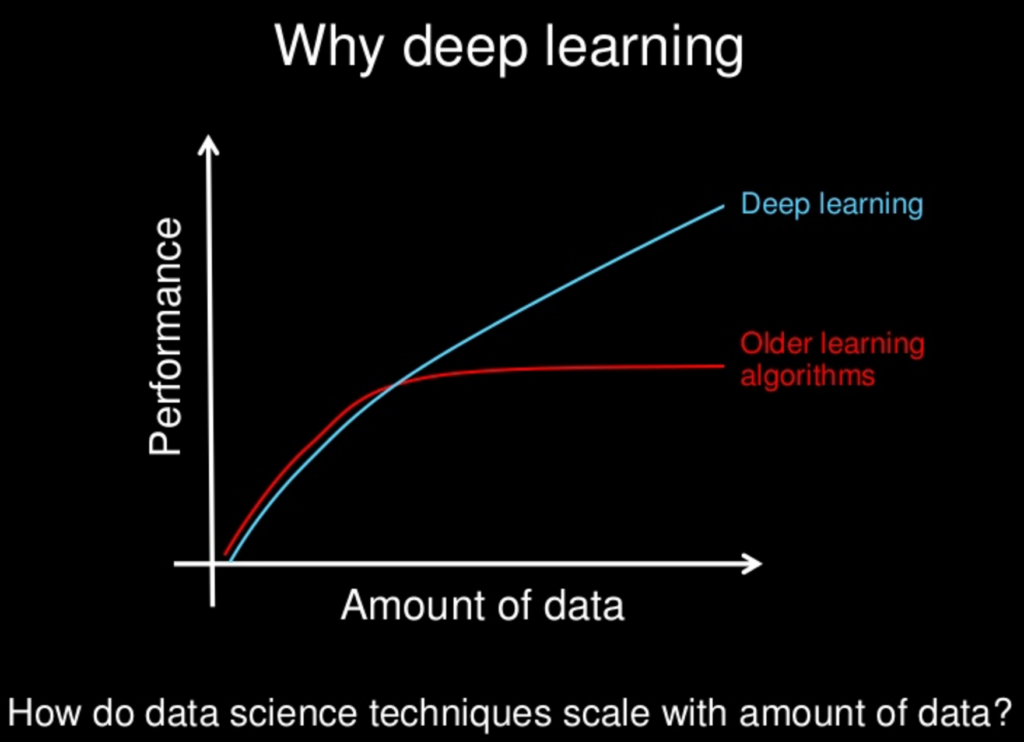
\includegraphics[width=.5\textwidth]{figures/whydeeplearning.png} 
\begin{itemize}
\item not memory-based
\item parallelizable computation(GPU optimizations)
\item many hyper-parameters but faster validation
\end{itemize}

\end{frame}

\begin{frame}
\frametitle{Motivations (2)}

\only<2->{
 \begin{textblock}{5}(5,5)
 \important{DEEP LEARNING}
 \end{textblock}
}
\textbf{Profiling phase}
\begin{itemize}
\item \only<1>{manage de-synchronization problem [$\setDataTrain \longrightarrow \rho\colon \mathbb{R}^D\rightarrow\mathbb{R}^D$]}\only<2->{\textcolor{gray}{manage de-synchronization problem [$\setDataTrain \longrightarrow \rho\colon \mathbb{R}^D\rightarrow\mathbb{R}^D$]}}
\item \only<1>{mandatory dimensionality reduction [$\setDataTrain \longrightarrow \extract\colon\mathbb{R}^D\rightarrow \mathbb{R}^C$]}
\only<2->{\textcolor{gray}{mandatory dimensionality reduction [$\setDataTrain \longrightarrow \extract\colon\mathbb{R}^D\rightarrow \mathbb{R}^C$]}}
\item estimate
\only<1>{
\begin{itemize}
\item $\pdf_{\given{\extract{(\rho(\vaLeakVec)})}{\sensRandVar = \sensVar}}$, $\pdf_{\extract{(\rho(\vaLeakVec)})}$, $\pdf_{\sensRandVar}$ (generative model)

\begin{itemize}
\item Gaussian hypothesis \cite{Chari2003}
\item Variants: \emph{pooled} version \cite{choudary2014efficient}, linear regression \cite{schindler2005stochastic}
\end{itemize}
\end{itemize}
}
\only<2->{
\begin{itemize}
\item \textcolor{gray}{$\pdf_{\given{\extract{(\rho(\vaLeakVec)})}{\sensRandVar = \sensVar}}$, $\pdf_{\extract{(\rho(\vaLeakVec)})}$, $\pdf_{\sensRandVar}$ (generative model)}
\begin{itemize}
\item \textcolor{gray}{ Gaussian hypothesis \cite{Chari2003}}
\item \textcolor{gray}{Variants: \emph{pooled} version \cite{choudary2014efficient}, linear regression \cite{schindler2005stochastic}}
\end{itemize}
\end{itemize}
}


\item $\pdf_{\given{\sensRandVar}{\only<1>{\extract{(\rho(\vLeakVec)}}  \only<2->{\vaLeakVec}}}$ (discriminative model) \\ \uncover<2->{by means of a neural network $F(\vaLeakVec)\approx \pdf_{\given{\sensRandVar}{ \only<2->{\vaLeakVec}}}$ (Universal approximation theorem)} 


\end{itemize}
\begin{block}{}
Many independent preprocessing steps and assumptions\\ \uncover<3>{$\longleftrightarrow$ integrated and agnostic approach}
\end{block}
\end{frame}


\begin{frame}
\frametitle{Multi-Layer Perceptron}
\begin{block}{Multi-Layer Perceptron (MLP)}
\only<1>{
$F(\vLeakVec,W) = \softmax\circ\lambda_n\circ\sigma_{n-1}\circ\lambda_{n-1}\circ\dots\circ \lambda_1(\vLeakVec)=\yyy \approx \mathrm{Pr}[\sensRandVar | \vaLeakVec = \vLeakVec] $
\begin{itemize}
\item[]\textcolor{white}{$\lambda_i$ linear functions (linear combinations of time samples) depending on some trainable weights $W$}
\item[]\textcolor{white}{$\sigma_i$ non-linear functions}
\item[]\textcolor{white}{$\softmax$ normalizing \emph{softmax} function}
\end{itemize}}
\only<2>{
$F(\vLeakVec,W) = \softmax\circ\textcolor{red}{\lambda_n}\circ\sigma_{n-1}\circ\textcolor{red}{\lambda_{n-1}}\circ\dots\circ \textcolor{red}{\lambda_1}(\vLeakVec)=\yyy \approx \mathrm{Pr}[\sensRandVar | \vaLeakVec = \vLeakVec]$
\begin{itemize}
\item[]\textcolor{red}{$\lambda_i$} linear functions (linear combinations of time samples) depending on some \textbf{trainable weights} $W$
\item[]\textcolor{white}{$\sigma_i$ non-linear functions}
\item[]\textcolor{white}{$\softmax$ normalizing \emph{softmax} function}
\end{itemize}}
\only<3>{
$F(\vLeakVec,W) = \softmax\circ\lambda_n\circ\textcolor{red}{\sigma_{n-1}}\circ\lambda_{n-1}\circ\dots\circ \lambda_1(\vLeakVec)=\yyy \approx \mathrm{Pr}[\sensRandVar | \vaLeakVec = \vLeakVec] $
\begin{itemize}
\item[]{$\lambda_i$ linear functions (linear combinations of time samples) depending on some \textbf{trainable weights} $W$}
\item[]\textcolor{red}{$\sigma_i$} non-linear \emph{activation} functions
\item[]\textcolor{white}{$\softmax$ normalizing \emph{softmax} function}
\end{itemize}}
\only<4->{
$F(\vLeakVec,W) = \textcolor{red}{\softmax}\circ\lambda_n\circ\sigma_{n-1}\circ\lambda_{n-1}\circ\dots\circ \lambda_1(\vLeakVec)=\yyy \approx \mathrm{Pr}[\sensRandVar | \vaLeakVec = \vLeakVec] $
\begin{itemize}
\item[]{$\lambda_i$ linear functions (linear combinations of time samples) depending on some \textbf{trainable weights} $W$}
\item[]{$\sigma_i$ non-linear \emph{activation} functions}
\item[]\textcolor{red}{$\softmax$} normalizing \emph{softmax} function
\end{itemize}}

\end{block}
\uncover<5->{
\begin{block}{Softmax $\sim$ multi-class logistic sigmoid}
\begin{equation}\label{eq:softmax}
\softmax(\aaa)[k] = \frac{e^{\aaa[k]}}{\sum_{j=1}^{\numClasses}e^{\aaa[j]}}\mbox{ .}
\end{equation}
\begin{equation}\label{eq:post_probs_multi-class}
\prob(\given{\sensVarValue{j}}{\vLeakVec})  = \frac{\prob(\given{\vLeakVec}{\sensVarValue{j}})\prob(\sensVarValue{j})}{\prob(\vLeakVec)} = \frac{\prob(\given{\vLeakVec}{\sensVarValue{j}})\prob(\sensVarValue{j})}{\sum_{k=1}^{\nbClasses}\prob(\given{\vLeakVec}{\sensVarValue{k}})\prob(\sensVarValue{k} )} = \softmax (\aaa)[j]\mbox{ ,}
\end{equation}
\end{block}
}
\end{frame}

\begin{frame}
\frametitle{Training-Validation-Test}
\only<1>{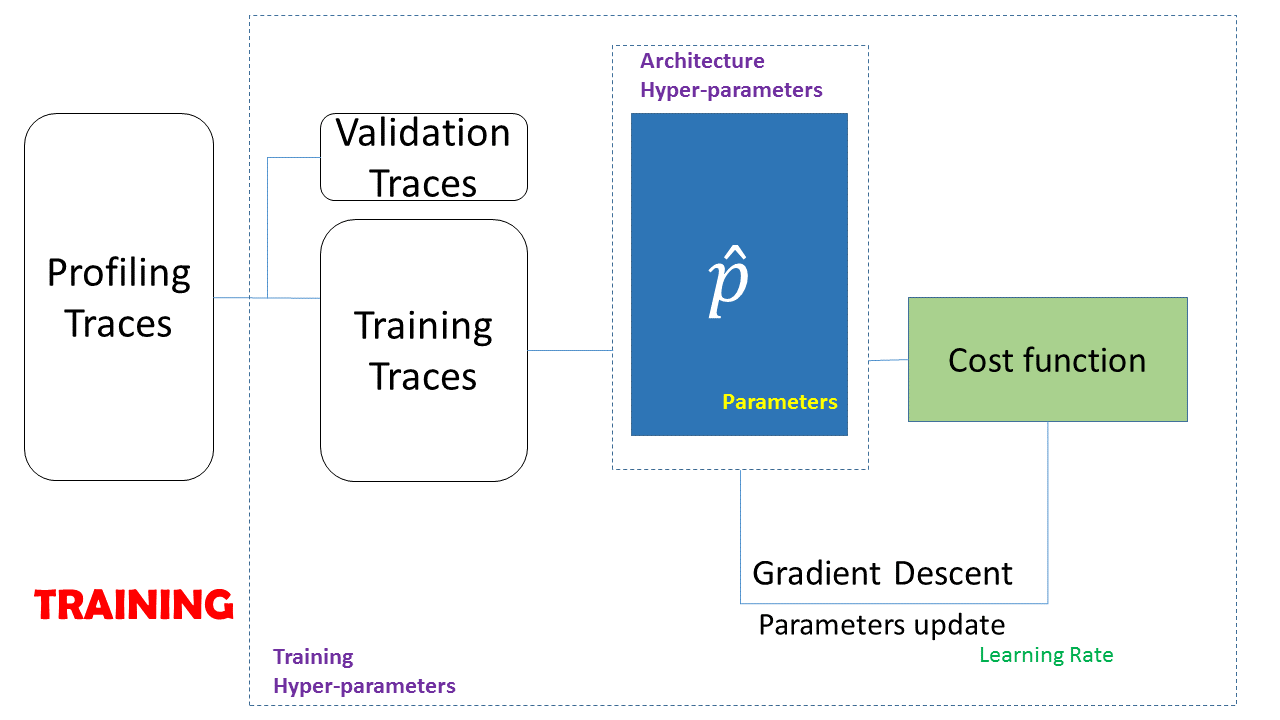
\includegraphics[width=\textwidth]{figures/deep_learning/Diapositive1.PNG}}
\only<2>{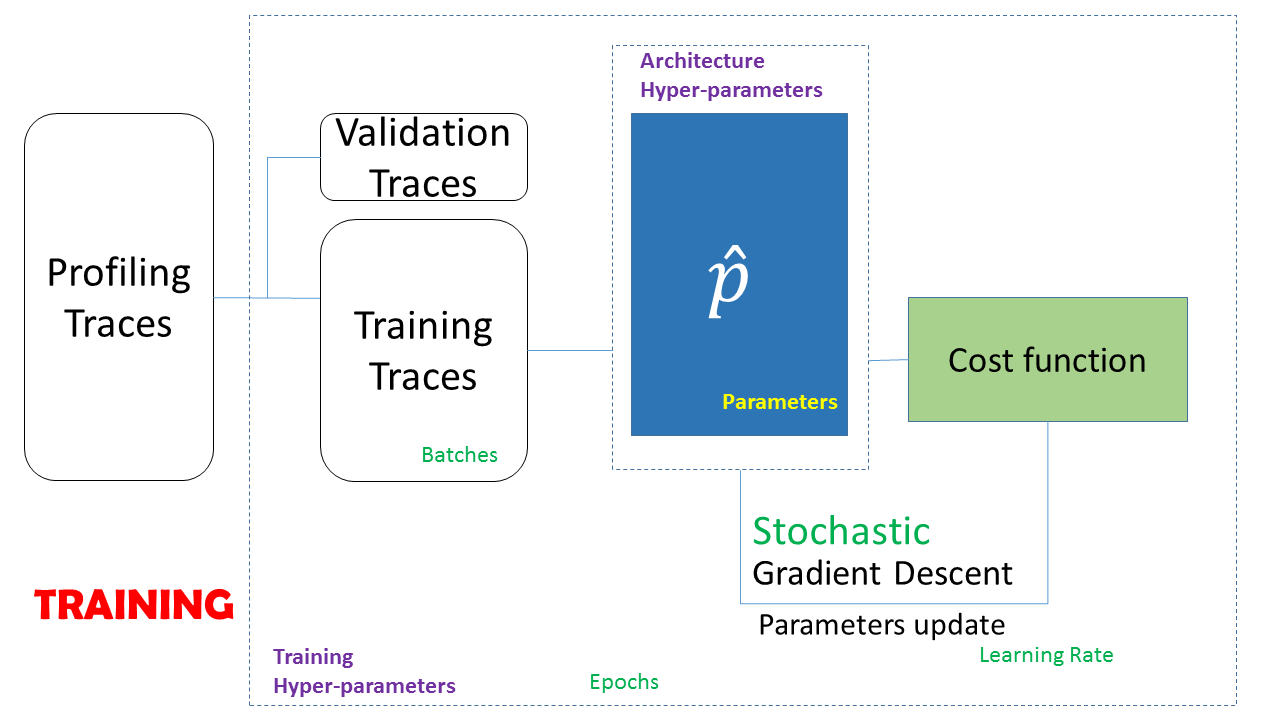
\includegraphics[width=\textwidth]{figures/deep_learning/Diapositive2.PNG}}
\only<3>{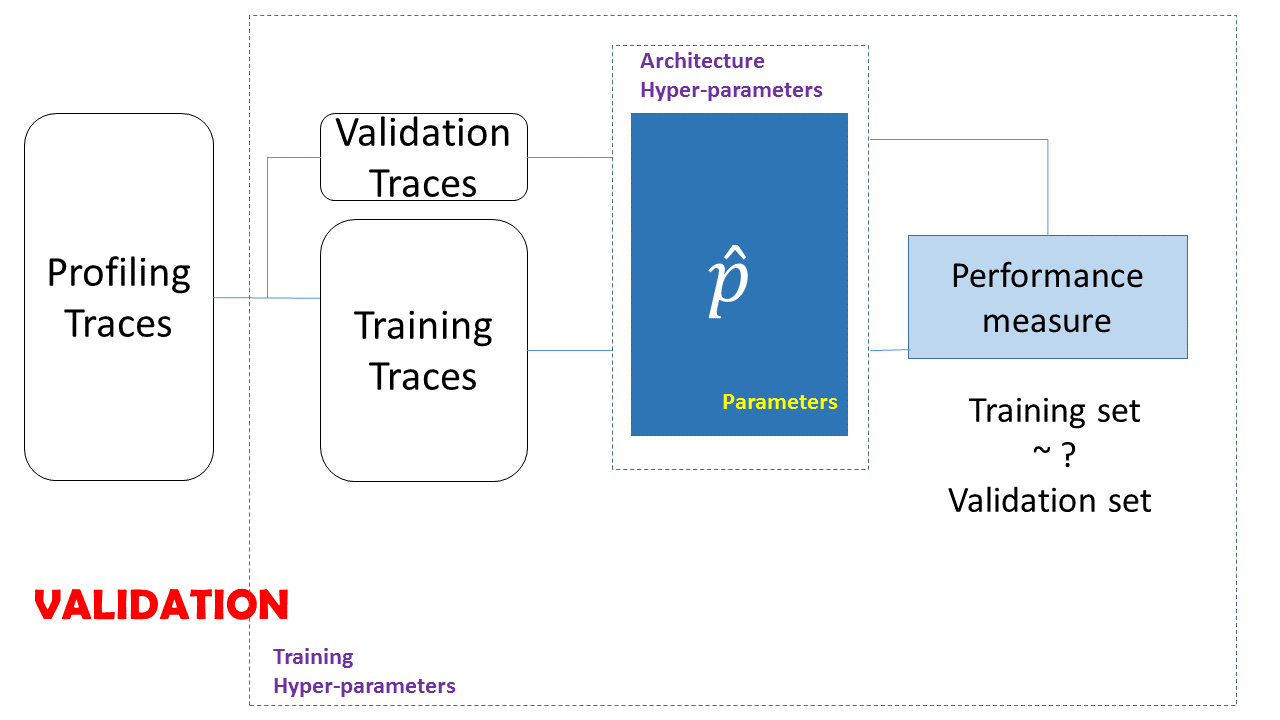
\includegraphics[width=\textwidth]{figures/deep_learning/Diapositive3.PNG}}
\only<4>{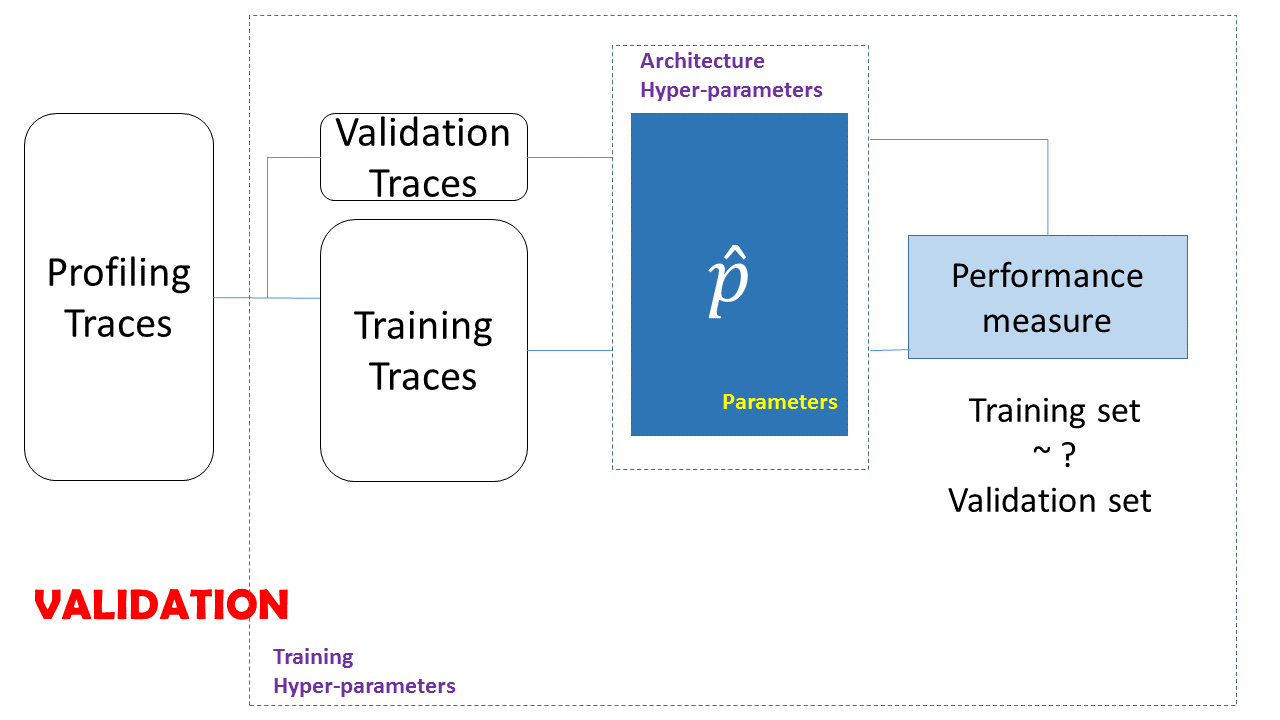
\includegraphics[width=\textwidth]{figures/deep_learning/Diapositive3.PNG}}
\end{frame}

\begin{frame}
\frametitle{Cost function - Cross-entropy}
\vspace*{-3pt}
\begin{itemize}
\item batch of training data $(\vLeakVec_i, \sensVar_i)_{i\in I}$, outputs of the current model $(\vNNOutput_i)_{i\in I}$
\item labels $\sensVar_i=\sensVarValue{j}$ are \emph{one-hot encoded}: $\vec{\sensVar_i} = \sensVarOneHot{j} = (0,\ldots , 0,\underbrace{1}_{j},0,\dots,0)$
\end{itemize}

\begin{block}{Loss function}
\begin{equation}\label{eq:lossfunction}
\mathcal{L} = -\frac{1}{\lvert I \rvert} \sum_{i\in I} \sum_{t=1}^{|\sensVarSet|}\vec{\sensVar_i}[t]\log{\vNNOutput_i[t]}
\end{equation}   
\end{block}

\begin{block}{Maximum-\emph{a-posteriori} or Cross-entropy}
\begin{itemize}
\item $\vNNOutput_i \approx \prob[\given{\sensRandVar}{\vaLeakVec=\vLeakVec_i}]$
\uncover<2>{\item $\vec{\sensVar_i} \approx \prob[\given{\sensRandVar}{\sensRandVar=\sensVarOneHot{j}}]$}
\uncover<2>{\item $\entropy(\vec{\sensVar_i}, \vNNOutput_i) = \entropy(\vec{\sensVar_i}) + D_{KL}(\vec{\sensVar_i} || \vNNOutput_i) = \esper_{\vec{\sensVar_i}}[-\log{\vNNOutput_i}] = -\sum_{t=1}^{|\sensVarSet|}\vec{\sensVar_i}[t]\log{\vNNOutput_i[t]}$}
\only<1>{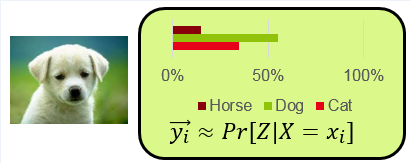
\includegraphics[width=0.4\textwidth]{figures/maxaposteriori.png}}
\only<2>{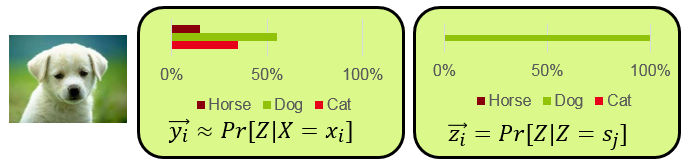
\includegraphics[width=0.7\textwidth]{figures/crossentropy.png}}
\end{itemize}
\end{block}
\end{frame}

\begin{frame}
\frametitle{Capacity-Overfitting-Regularization}


\begin{block}{Regression example}
Performance metric: Mean Square Error (MSE)
\begin{columns}
\begin{column}{.5\textwidth}
\only<1-2>{\begin{figure}
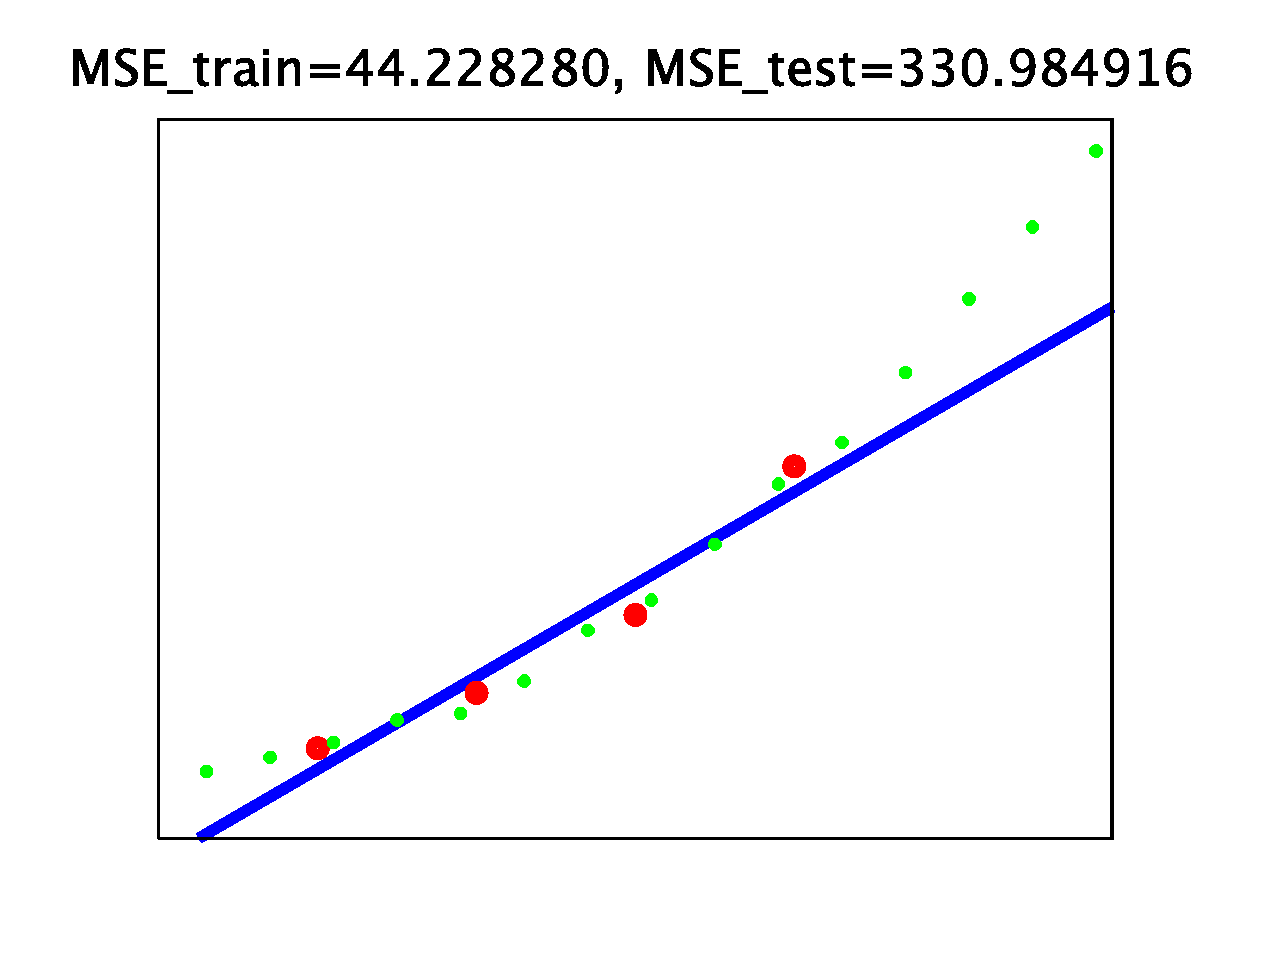
\includegraphics[width=\textwidth]{../Figures/linear_regression.pdf}
\caption{Linear regression $\rightarrow$ underfitting}
\end{figure}}
\only<3-4>{\begin{figure}
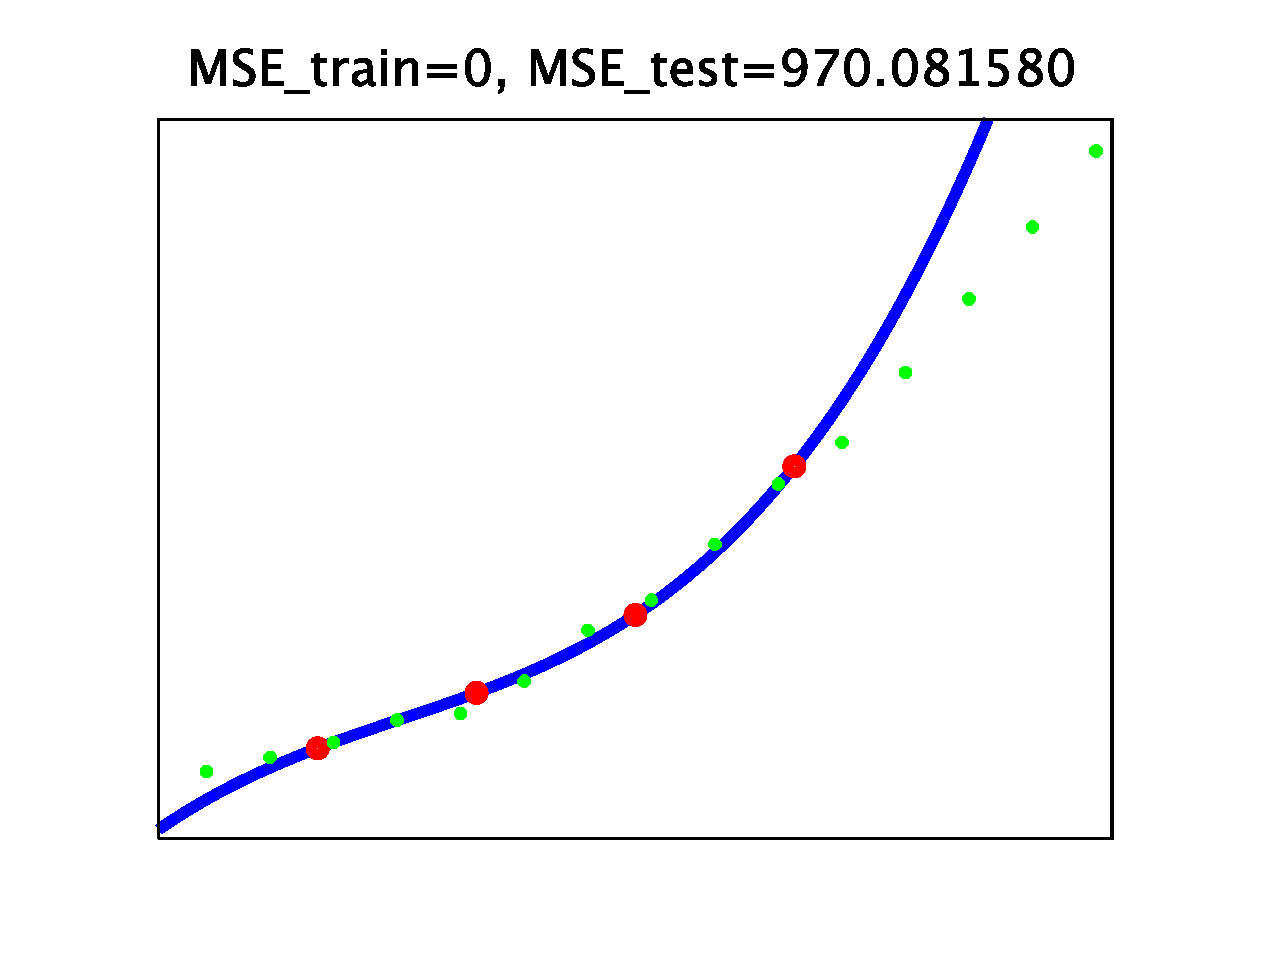
\includegraphics[width=\textwidth]{../Figures/cubic_regression.pdf}
\caption{Cubic regression $\rightarrow$ overfitting}
\end{figure}}
\end{column}
\begin{column}{.5\textwidth}
\only<2-3>{
\begin{figure}
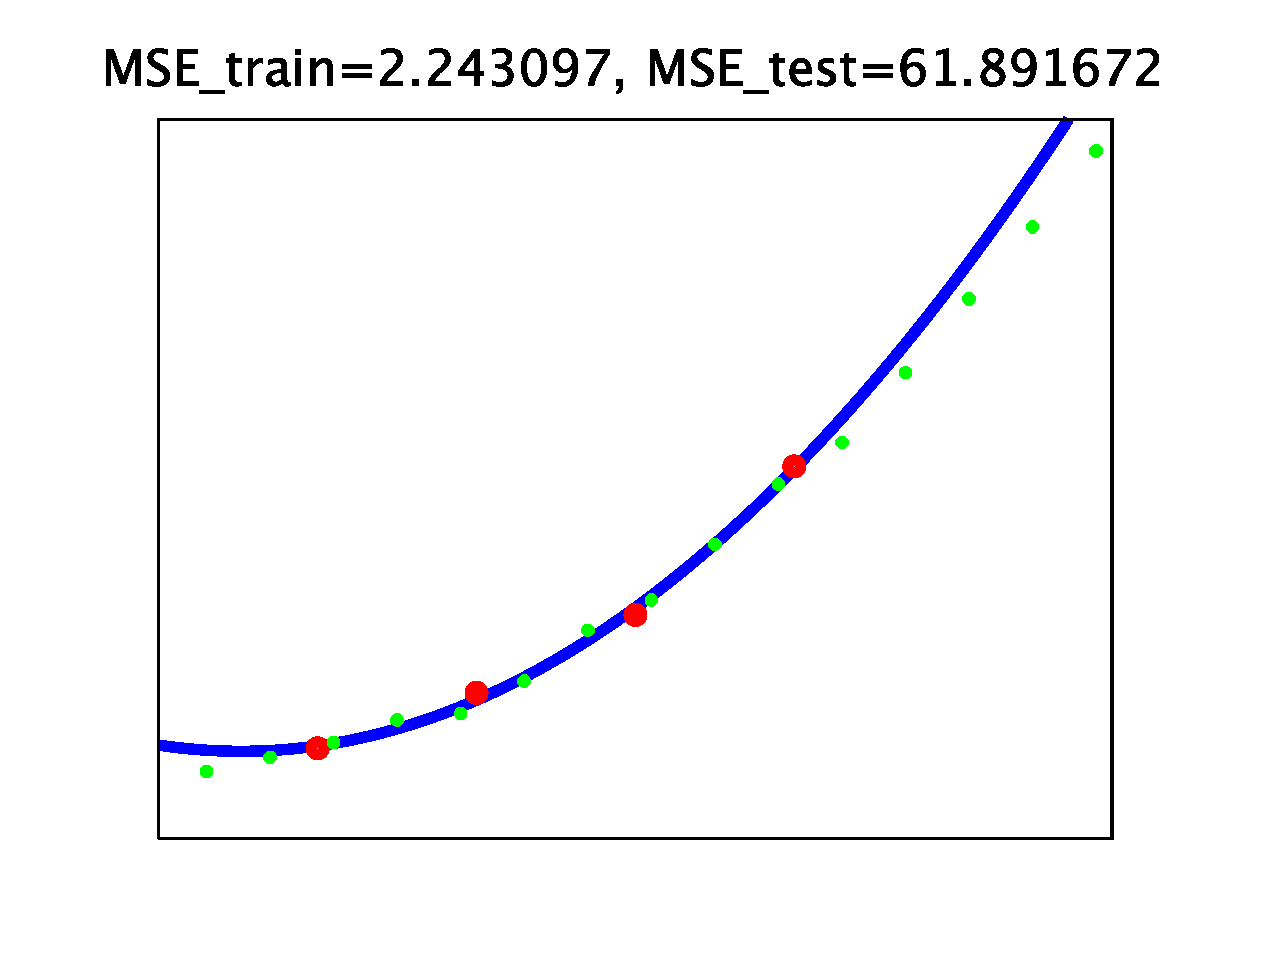
\includegraphics[width=\textwidth]{../Figures/quadratic_regression.pdf}
\caption{Linear regression $\rightarrow$ fits}
\end{figure}}
\only<4>{
\begin{figure}
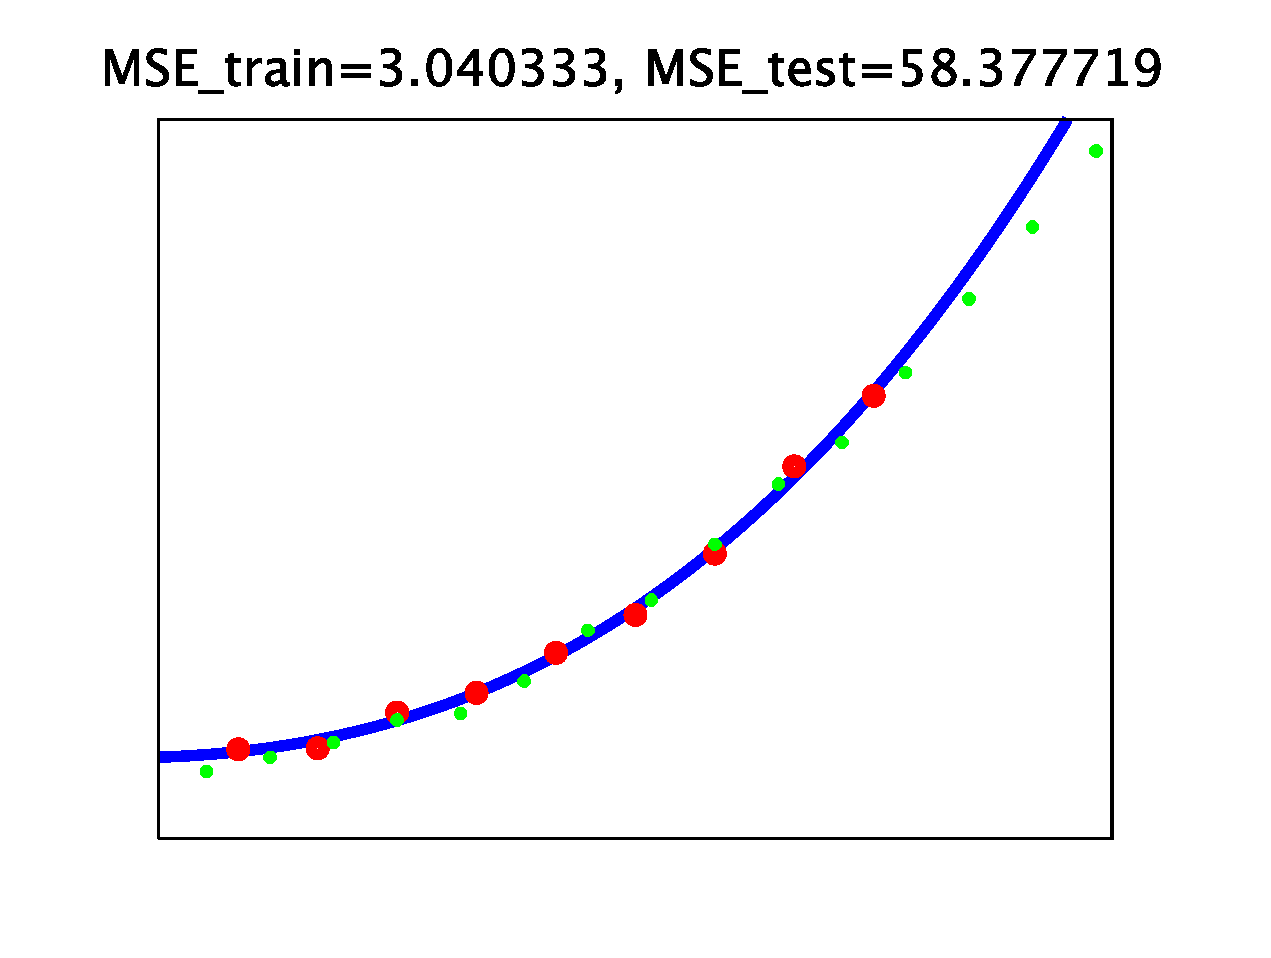
\includegraphics[width=\textwidth]{../Figures/cubic_regression_more.pdf}
\caption{Cubic regression with more training data}
\end{figure}}
\end{column}
\end{columns}
\end{block}

\uncover<5->{
\begin{block}{Classification via Neural Network}
Performance measure: Accuracy (Classification rate)\\
Evaluate and compare training and validation accuracy
\begin{columns}
\begin{column}{.45\textwidth}
\only<5>{Understand significant features
\begin{figure}
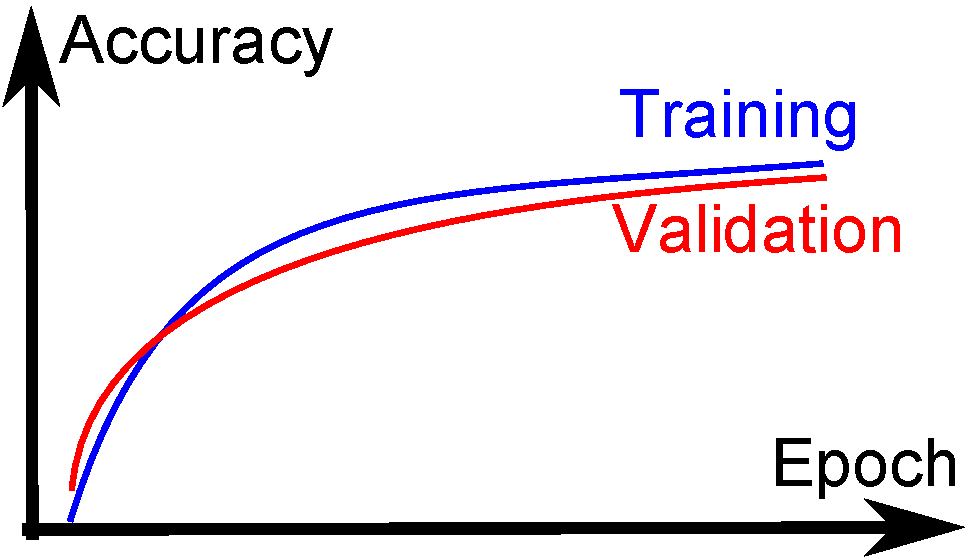
\includegraphics[width=.9\textwidth]{figures/fitting.pdf} 
\end{figure}
}
\only<6>{
Why?
\begin{itemize}
\item[] Too complex model
\item[] Not enough training data
\end{itemize}
Solution? 
\begin{itemize}
\item[] Data augmentation
\end{itemize}
}
\end{column}
\begin{column}{.45\textwidth}
Learn by heart (\textbf{\textcolor{red}{OVERFITTING}})
\begin{figure}
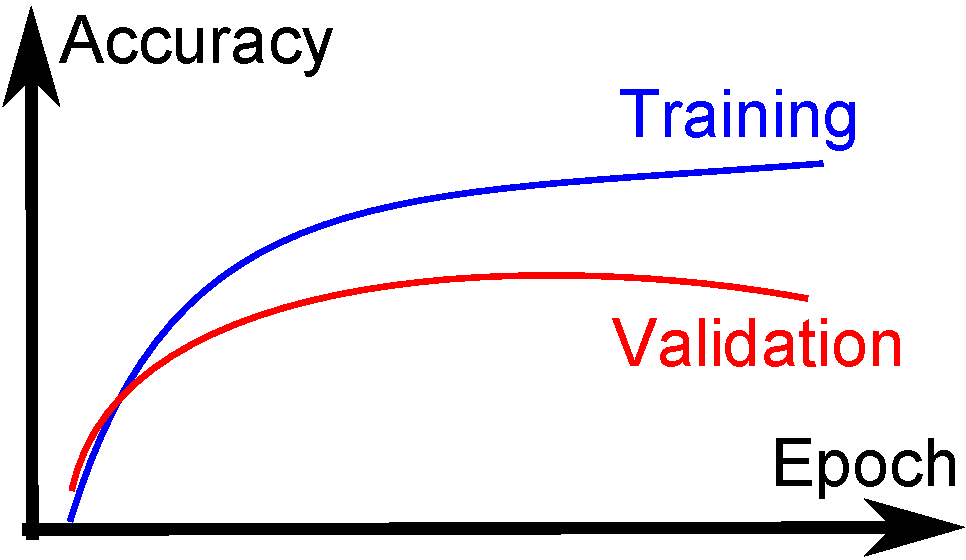
\includegraphics[width=.9\textwidth]{figures/overfitting.pdf} 
\end{figure}

\end{column}
\end{columns}
\end{block}

}



\end{frame}

%
\begin{frame}
\frametitle{Convolutional Neural Networks}
\begin{block}{Translation-invariance}
\begin{figure}
\centering
\only<1>{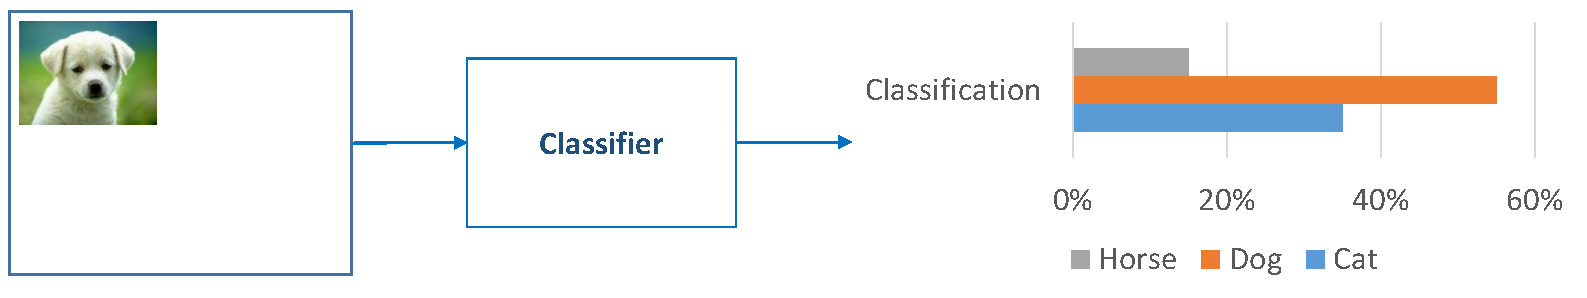
\includegraphics[width=\textwidth]{Figures/cane_shift_classifier1.pdf}}
\only<2>{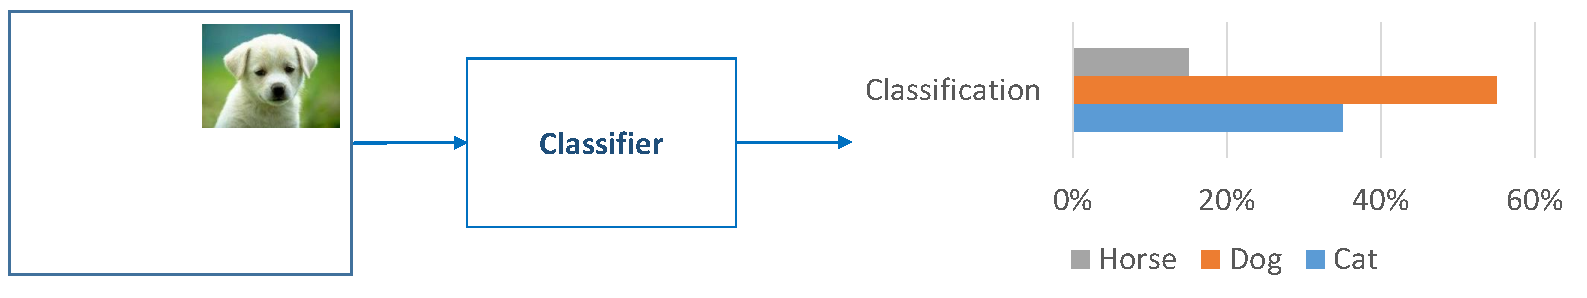
\includegraphics[width=\textwidth]{Figures/cane_shift_classifier2.pdf}}
\only<3-4>{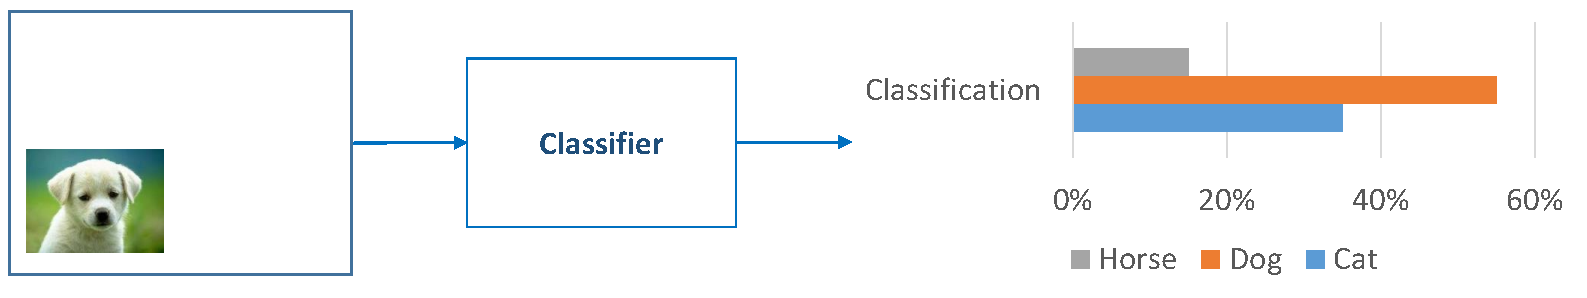
\includegraphics[width=\textwidth]{Figures/cane_shift_classifier3.pdf}}
\only<5>{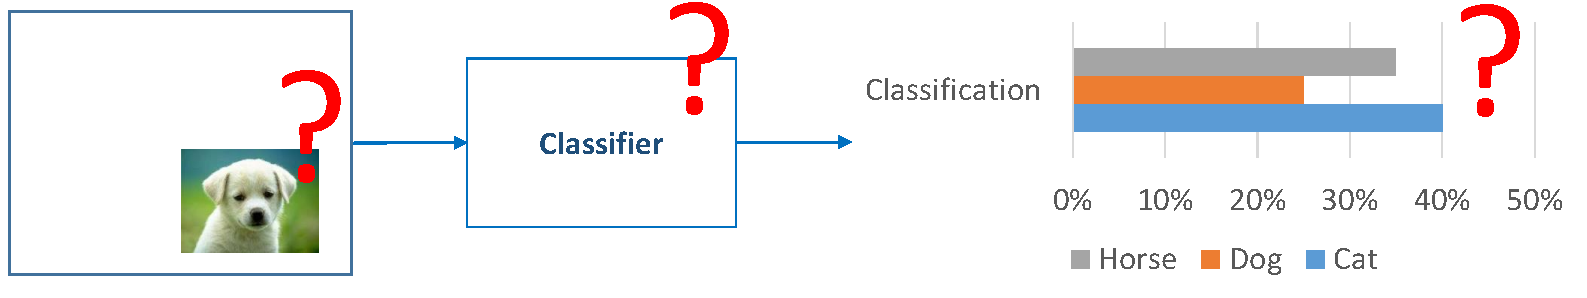
\includegraphics[width=\textwidth]{Figures/cane_shift_classifier4.pdf}}
\only<6>{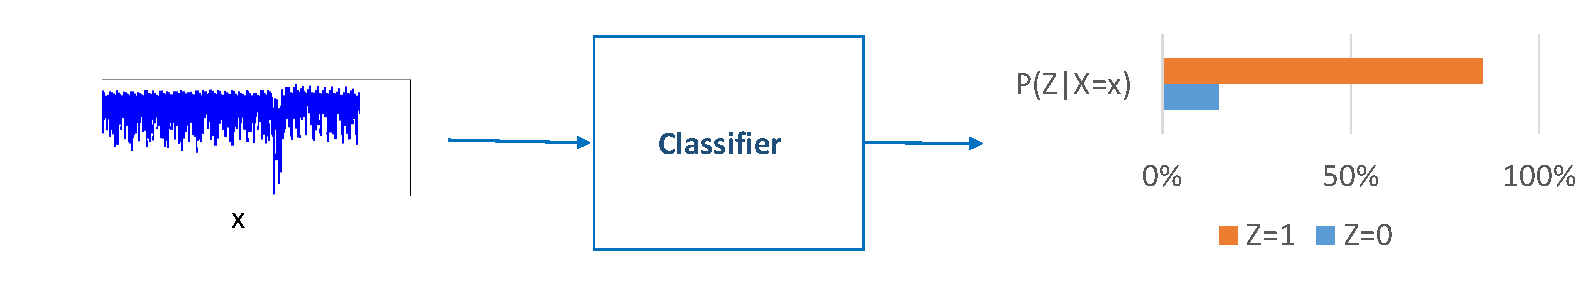
\includegraphics[width=\textwidth]{Figures/trace_shift_classifier1.pdf}}
\only<7>{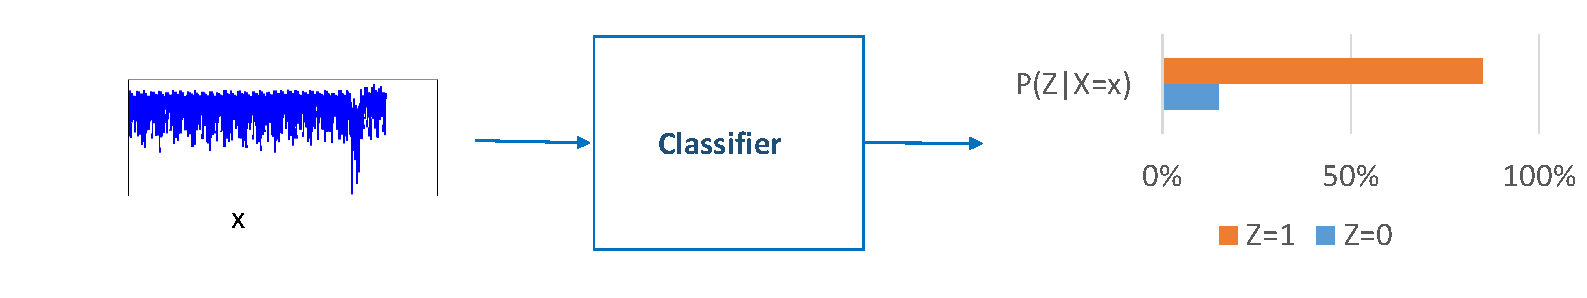
\includegraphics[width=\textwidth]{Figures/trace_shift_classifier2.pdf}}
\only<8->{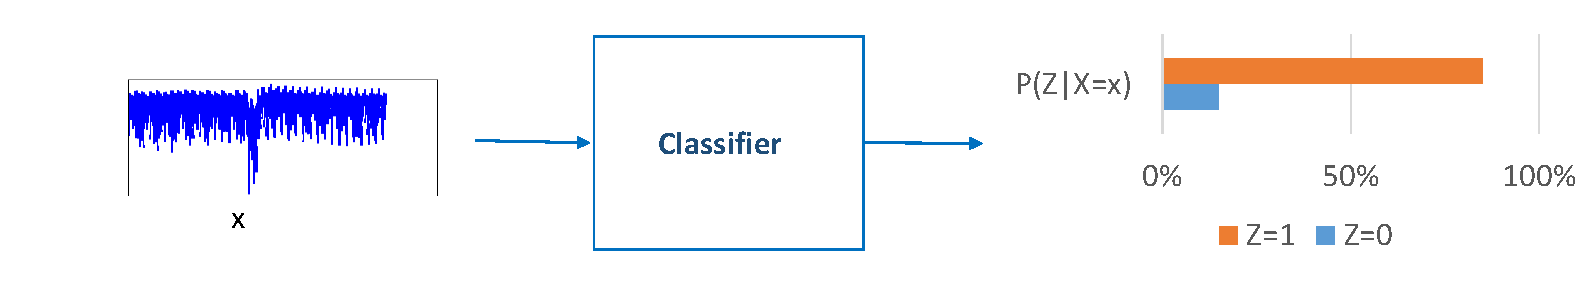
\includegraphics[width=\textwidth]{Figures/trace_shift_classifier3.pdf}}
\end{figure}
\uncover<4->{It is important to explicit the data translation-invariance\\}
\uncover<9->{Convolutional Neural Networks: share weights across space}
\end{block}
%

\vspace*{-7pt}

\begin{columns}
\begin{column}{.5\textwidth}
\only<1-10>{
\begin{figure}

\includegraphics[width=.7\textwidth]{Figures/small_white.pdf}
\end{figure}
}

\only<11>{
\begin{figure}
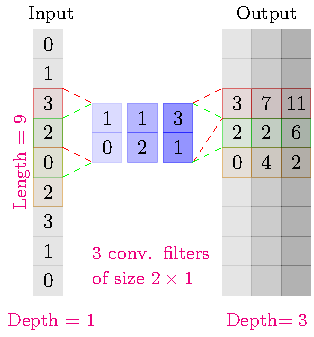
\includegraphics[width=.6\textwidth]{../tikz_per_manuscritto/conv_filter_2_1.pdf} 
\caption{\scriptsize{Linear layer in a ConvNet (\emph{Convolutional Layer})}}
\end{figure}
}

\only<12>{
\begin{figure}
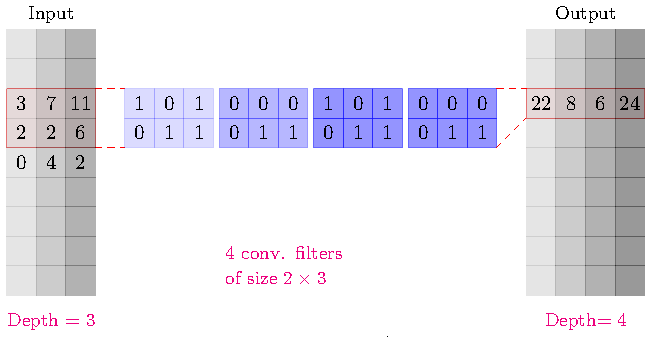
\includegraphics[width=0.8\textwidth]{../tikz_per_manuscritto/conv_filter_2_3.pdf} 
\caption{\scriptsize{Linear layer in a ConvNet (\emph{Convolutional Layer})}}
\end{figure}
}

\end{column}
%%
\begin{column}{.5\textwidth}
\only<1-9>{
\begin{figure}

\includegraphics[width=.7\textwidth]{Figures/big_white.pdf}
\end{figure}}
\only<10-12>{
\begin{figure}
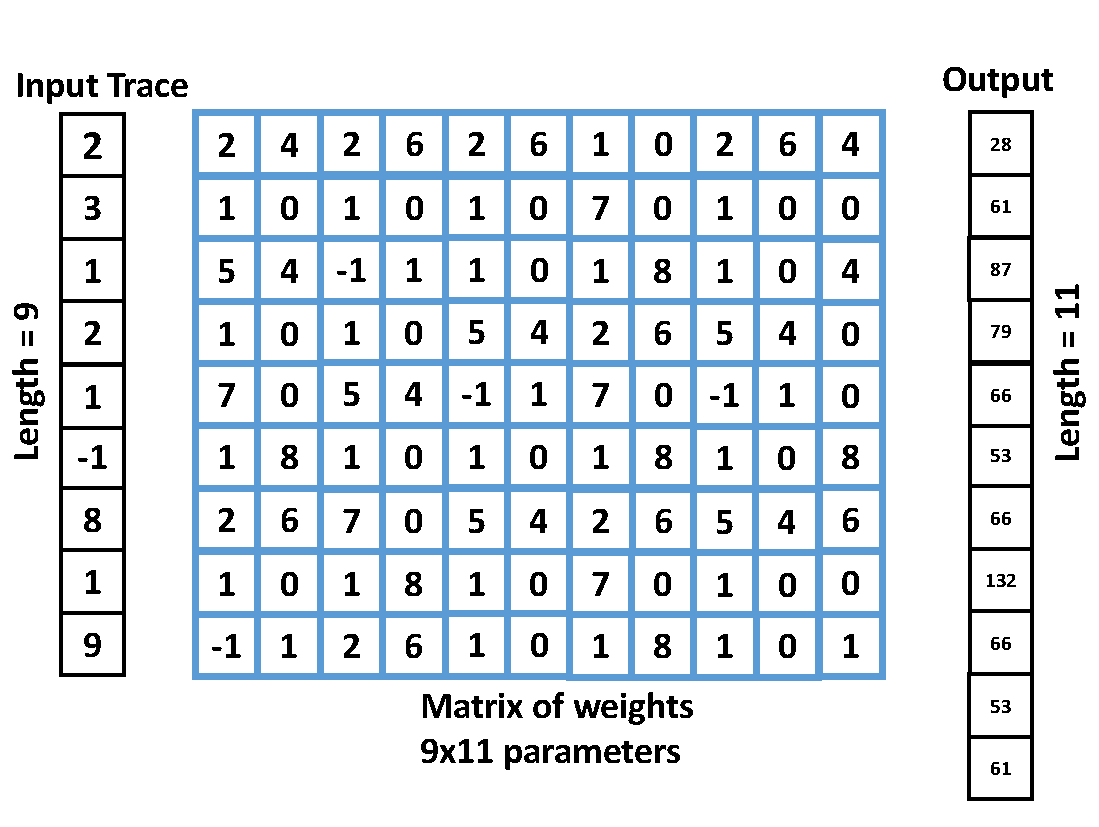
\includegraphics[width=.8\textwidth]{Figures/FC.pdf} 
\caption{\scriptsize{Linear layer in an MLP (\emph{Fully Connected Layer})}}
\end{figure}
}
\only<14->{
\begin{figure}
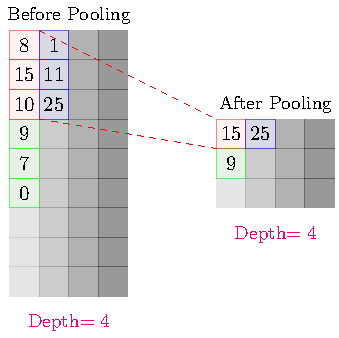
\includegraphics[width=.6\textwidth]{../tikz_per_manuscritto/pooling.pdf} 
\caption{\scriptsize{Max Pooling Layer}}
\end{figure}
}

\end{column}
\end{columns}
\end{frame}


\begin{frame}
\frametitle{A kind of CNN architecture}
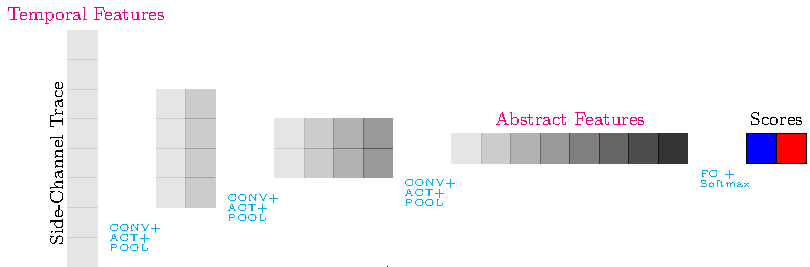
\includegraphics[width=\textwidth]{../tikz_per_manuscritto/convnet_arch.pdf} \\VGG-like:
\begin{itemize}
\item Reduce temporal features to only one
\item Maintain time complexity of each layer (one-half pooling when number of feature maps are doubled)
\item Small filters
\end{itemize}
\begin{block}{Model used in our experiments}
$\softmax \circ [\lambda]^1 \circ[\delta \circ [\sigma \circ \gamma  ]^1 ]^4$
\end{block}

\end{frame}


\subsection{Data Augmentation}
\begin{frame}
\frametitle{Data Augmentation}
\vspace{-11pt}
\begin{block}{Data Augmentation}
Artificially generate new training data by deforming those previously acquired,
Applying transformations that preserve the label $\sensRandVar$
\end{block}
\vspace{-5pt}
\begin{block}{Countermeasure Emulation Idea}
Emulate the effects of misaligning countermeasures to generate new traces
\begin{columns}
\begin{column}{0.35\textwidth}
\begin{large}
\textbf{\textcolor{green}{SHIFTING}}
\vspace{-8pt}
\end{large}
\end{column}
\begin{column}{0.35\textwidth}
\begin{large}
\textbf{\textcolor{blue}{ADD-REMOVE}}
\vspace{-8pt}
\end{large}
\end{column}
\end{columns}
\begin{figure}
  \begin{minipage}[b]{0.5\linewidth}
    \centering
    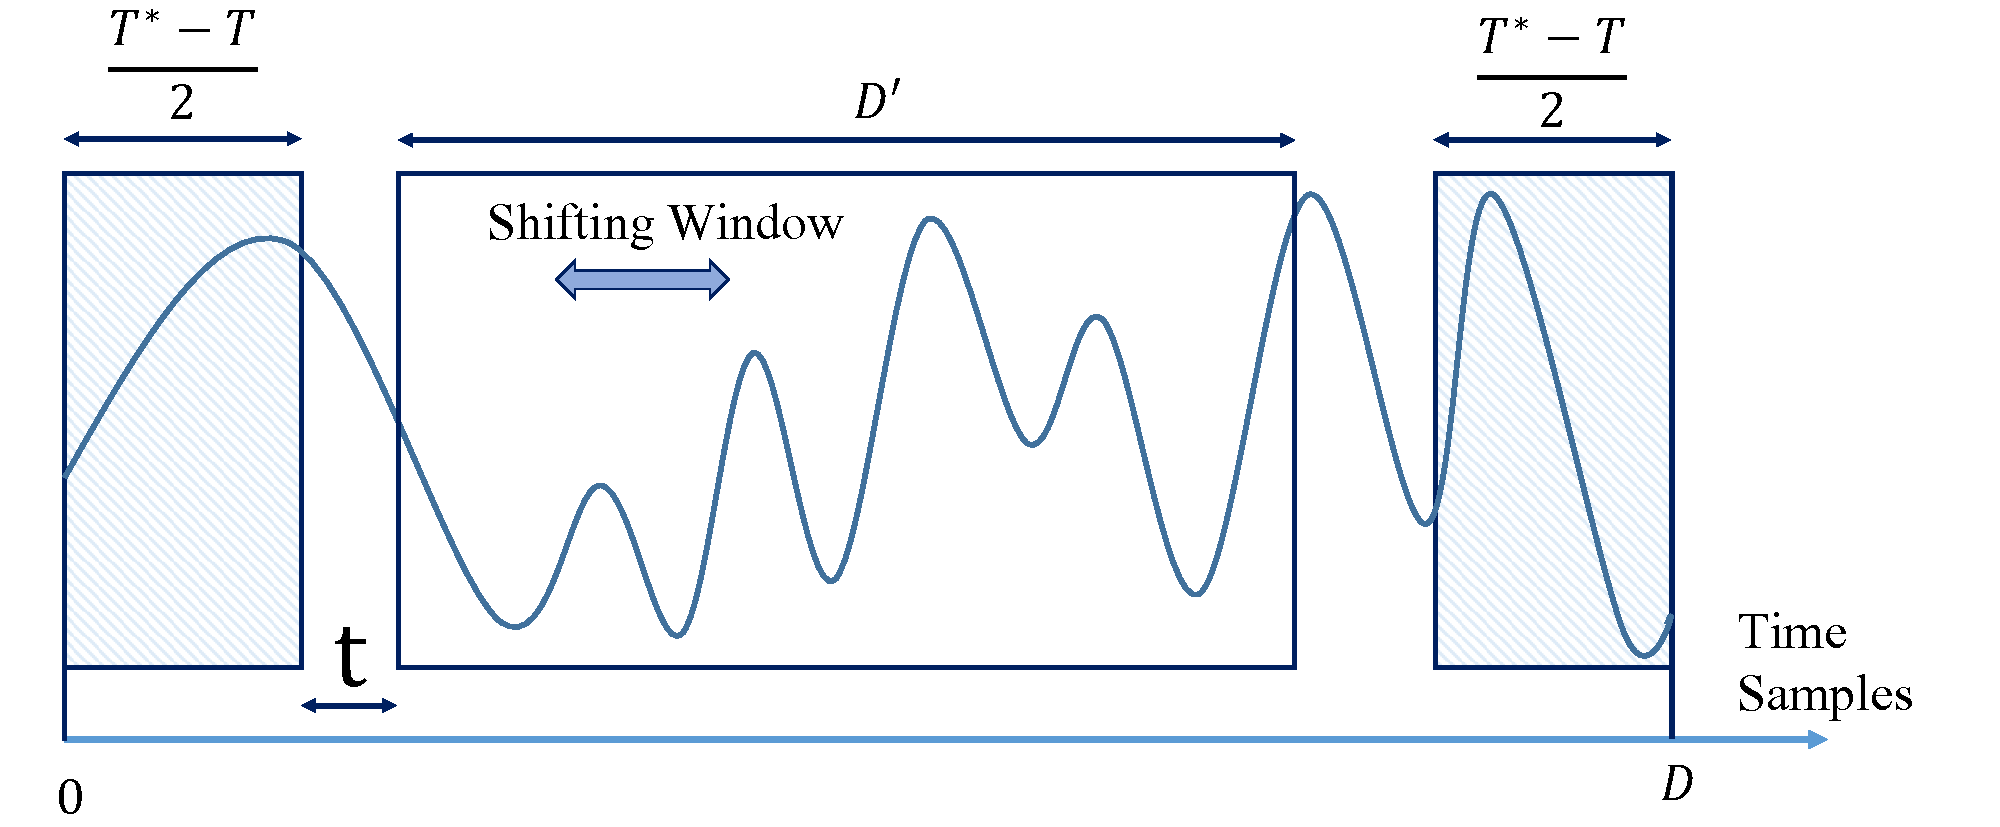
\includegraphics[width=\linewidth]{../Figures/CHES2017/Shifting_window.pdf} 
    \caption{\textcolor{green}{$SH_T$}}
  \end{minipage}%%
  \begin{minipage}[b]{0.5\linewidth}
    \centering
    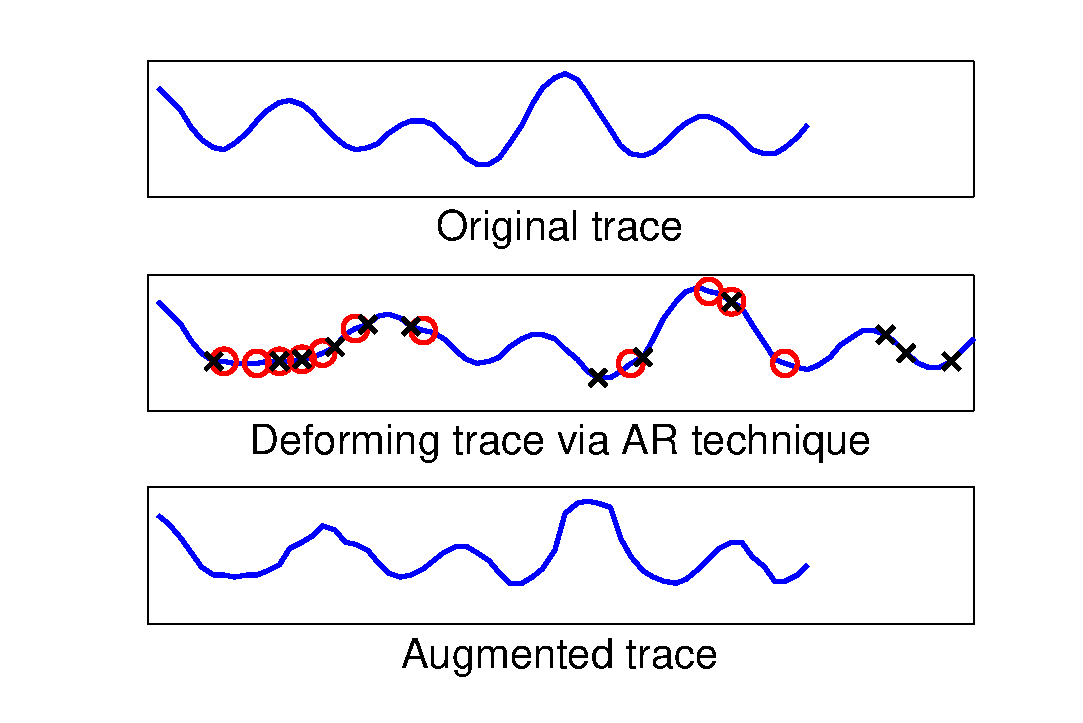
\includegraphics[width=.7\linewidth]{../Figures/CHES2017/AR_example.pdf} 
    \caption{\textcolor{blue}{$AR_R$}}
  \end{minipage} 
\end{figure}
\vspace{-9pt}
Parameter  \textcolor{green}{$T$}: $\sharp$ of possible positions \hfill \only<2->{\textcolor{red}{\small{$\longrightarrow$ new hyper-parameter}}}\\
Parameter \textcolor{blue}{$R$}: $\sharp$ of added and removed points \hfill \only<2->{\textcolor{red}{\small{$\longrightarrow$ new hyper-parameter}}}\\
Data Augmentation techniques are applied online during training phase.
\end{block}
\end{frame}


\subsection{Experimental Results}
\begin{frame}
\frametitle{Experimental Results}
\begin{itemize}
%\item \only<1-2>{Random delays}\only<3>{\textcolor{red}{Random delays}}
%\item \only<1-2>{Artificial Jitter}\only<3>{\textcolor{grey}{Artificial Jitter}}
%\item \only<1-2>{Real Jitter}\only<3>{\textcolor{red}{Real Jitter}}
\item Random delays
\item Artificial Jitter
\item Real Jitter
\end{itemize}

\vspace*{3pt}
Keras 1.2.1 library with Tensorflow backend \cite{keras} (open source, today 2.2.4)


\end{frame}

\begin{frame}
\vspace*{-5pt}
\frametitle{Random delays}
\vspace{-18pt}
\begin{figure}
\subfloat[One leaking operation]{
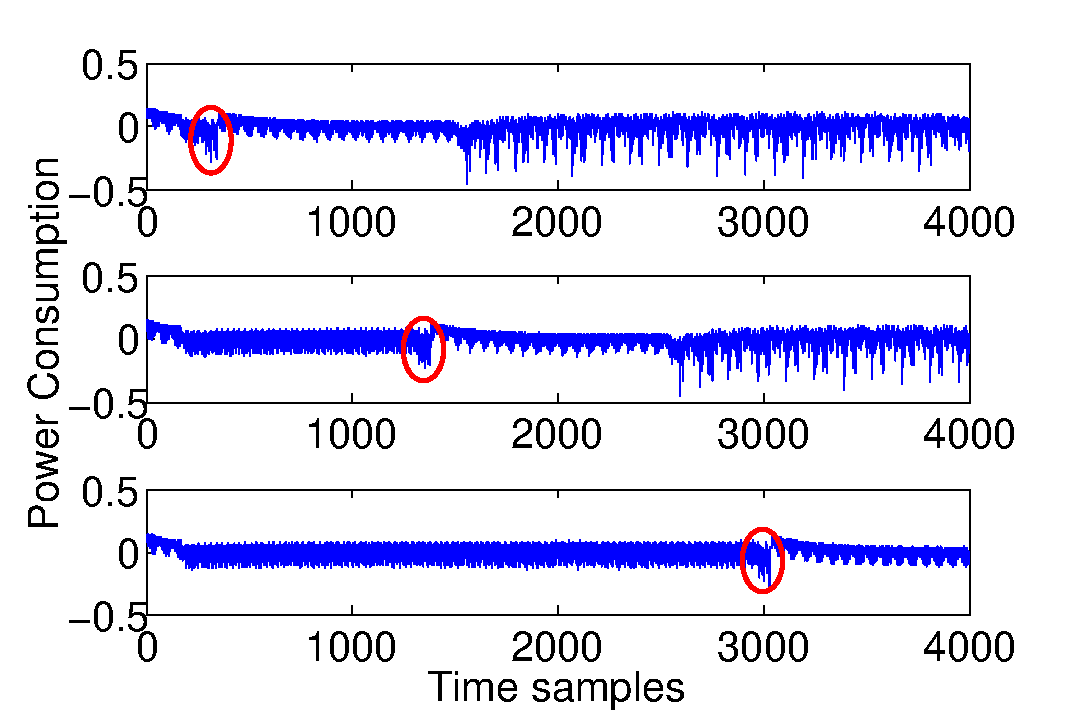
\includegraphics[width=.4\textwidth]{../Figures/CHES2017/CW_shift_traces.pdf} }

\end{figure}
\vspace*{-13pt}
\begin{block}{Setup}

\begin{itemize}
\item Target Chip: Atmega328P 
\item Target Variable: $Z = \mathrm{HW}(\mathrm{Sbox}(P\oplus K))$
\item Acquisition: through \emph{ChipWhisperer}\textregistered\ platform, $\approx 4,000$ time samples
\item Countermeasure: Random Delays - insertion of $r$ \emph{nop} operations, $r \in [0,127]$ uniform random
\item $1,000$ training traces

\end{itemize}
\end{block}


\end{frame}

\begin{frame}
\frametitle{Random delays}
\framesubtitle{Data augmentation vs overfitting}
\vspace{-8pt}
\begin{block}{Metrics}
\begin{itemize}
\item Test accuracy: classification accuracy over the attack traces
\item $N^\star$: minimum number of attack traces to make \emph{guessing entropy} of the right key permanently equal to one ($N^\star$ estimated over 10 independent attacks)
\end{itemize}
\end{block}


\begin{figure}
\captionsetup[subfigure]{labelformat=empty}
\subfloat[\textcolor{green}{$SH_0$}]{
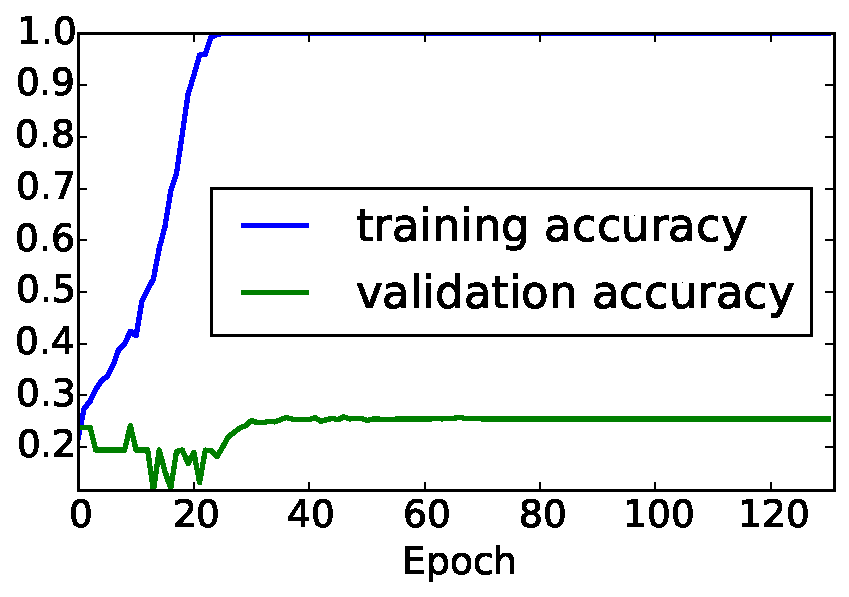
\includegraphics[width=.3\textwidth]{../Figures/CHES2017/DAshift0_2000traces_9classes_sgd/acc_DAshift0_2000traces_9classes_sgd.pdf} 
}
\subfloat[\textcolor{green}{$SH_{100}$}]{
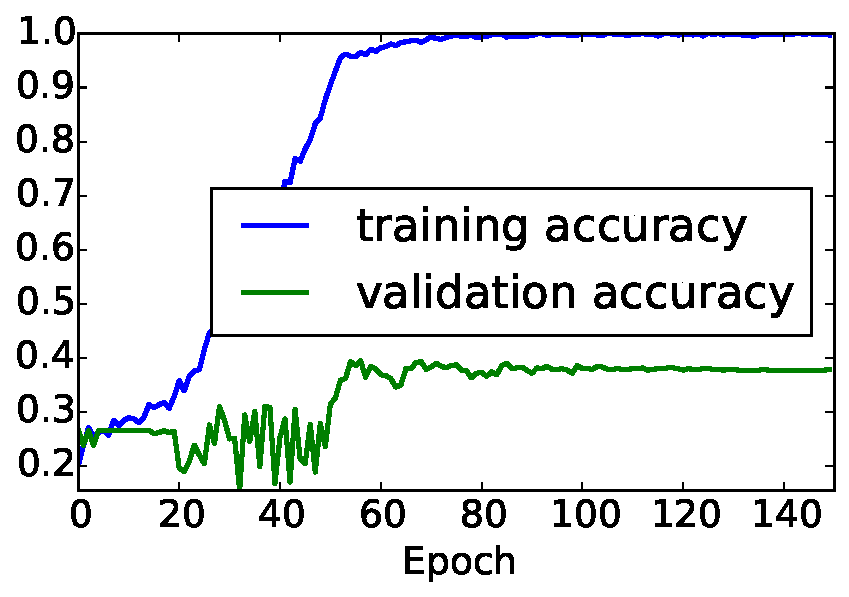
\includegraphics[width=.3\textwidth]{../Figures/CHES2017/DAshift100_2000traces_9classes_sgd/acc_DAshift100_2000traces_9classes_sgd.pdf} 
}
\subfloat[\textcolor{green}{$SH_{500}$}]{
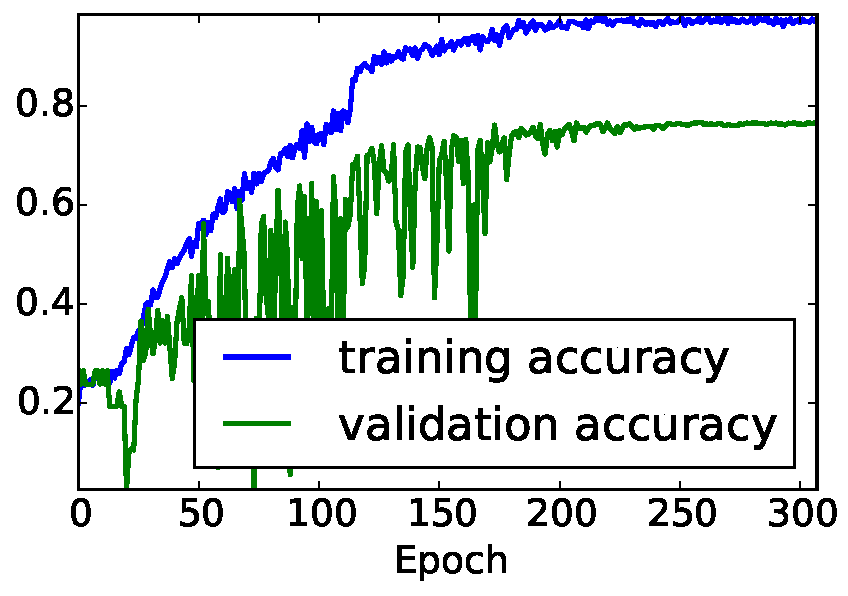
\includegraphics[width=.3\textwidth]{../Figures/CHES2017/DAshift500_2000traces_9classes_sgd/acc_DAshift500_2000traces_9classes_sgd.pdf} 
}
\end{figure}

\pause
\vspace*{-15pt}
\begin{table}
\begin{tabular}{|c|c|c|c|c|c|c|c|}
\multicolumn{8}{c}{}\\
\hline
\multicolumn{2}{|c|}{} & \multicolumn{2}{c|}{\textcolor{green}{$\mathrm{SH}_{0}$}} & \multicolumn{2}{c|}{\textcolor{green}{$\mathrm{SH}_{100}$}} & \multicolumn{2}{c|}{\textcolor{green}{$\mathrm{SH}_{500}$}} \\ \hline
Acc        & $N^\star$       & 27.0\%                      & $>1,000$                      & 31.8\%                       & 101                         & \textbf{78\%}              & \textbf{7}                \\ \hline
\end{tabular}
\end{table}
%
\end{frame}
%

\begin{frame}
\frametitle{Random Delays - Two Leaking Operations}

\centering
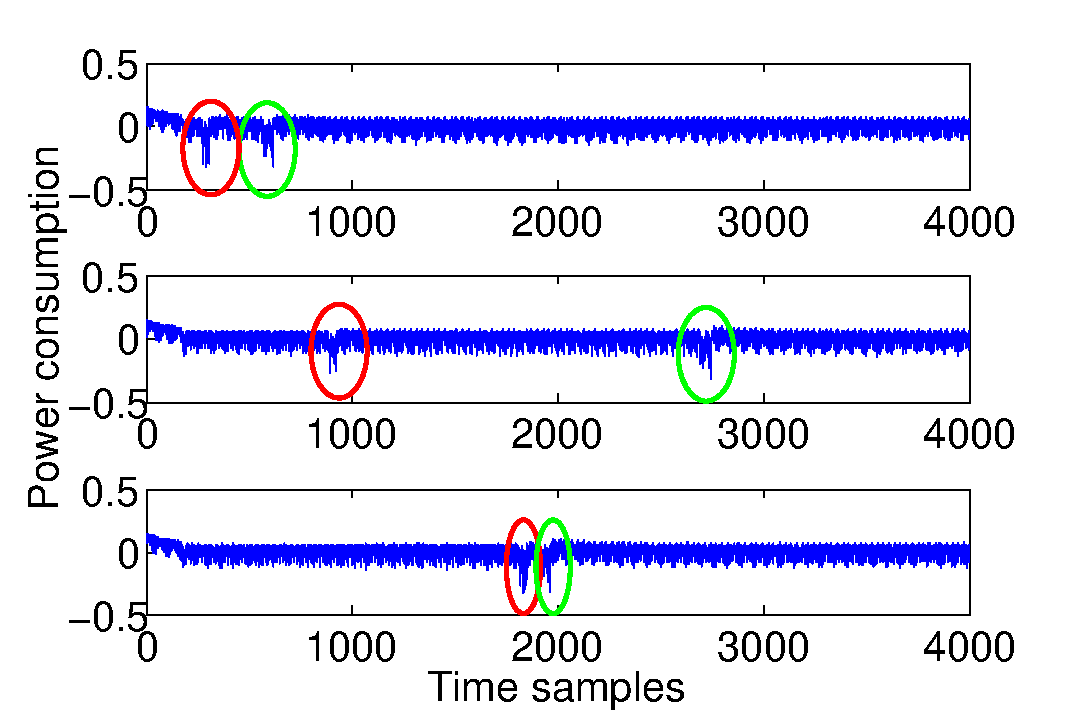
\includegraphics[width=.5\textwidth]{../Figures/CHES2017/CW_double_shift_traces.pdf}	


\begin{block}{Two leaking operations}
First operation - Test acc: $76.8\%$, $N^\star=7$\\
Second operation - Test acc: $82.5\%$, $N^\star=6$
\end{block}

\end{frame}

\begin{frame}
\frametitle{Artificial Jitter}
\begin{figure}
\subfloat[Low artificial jitter]{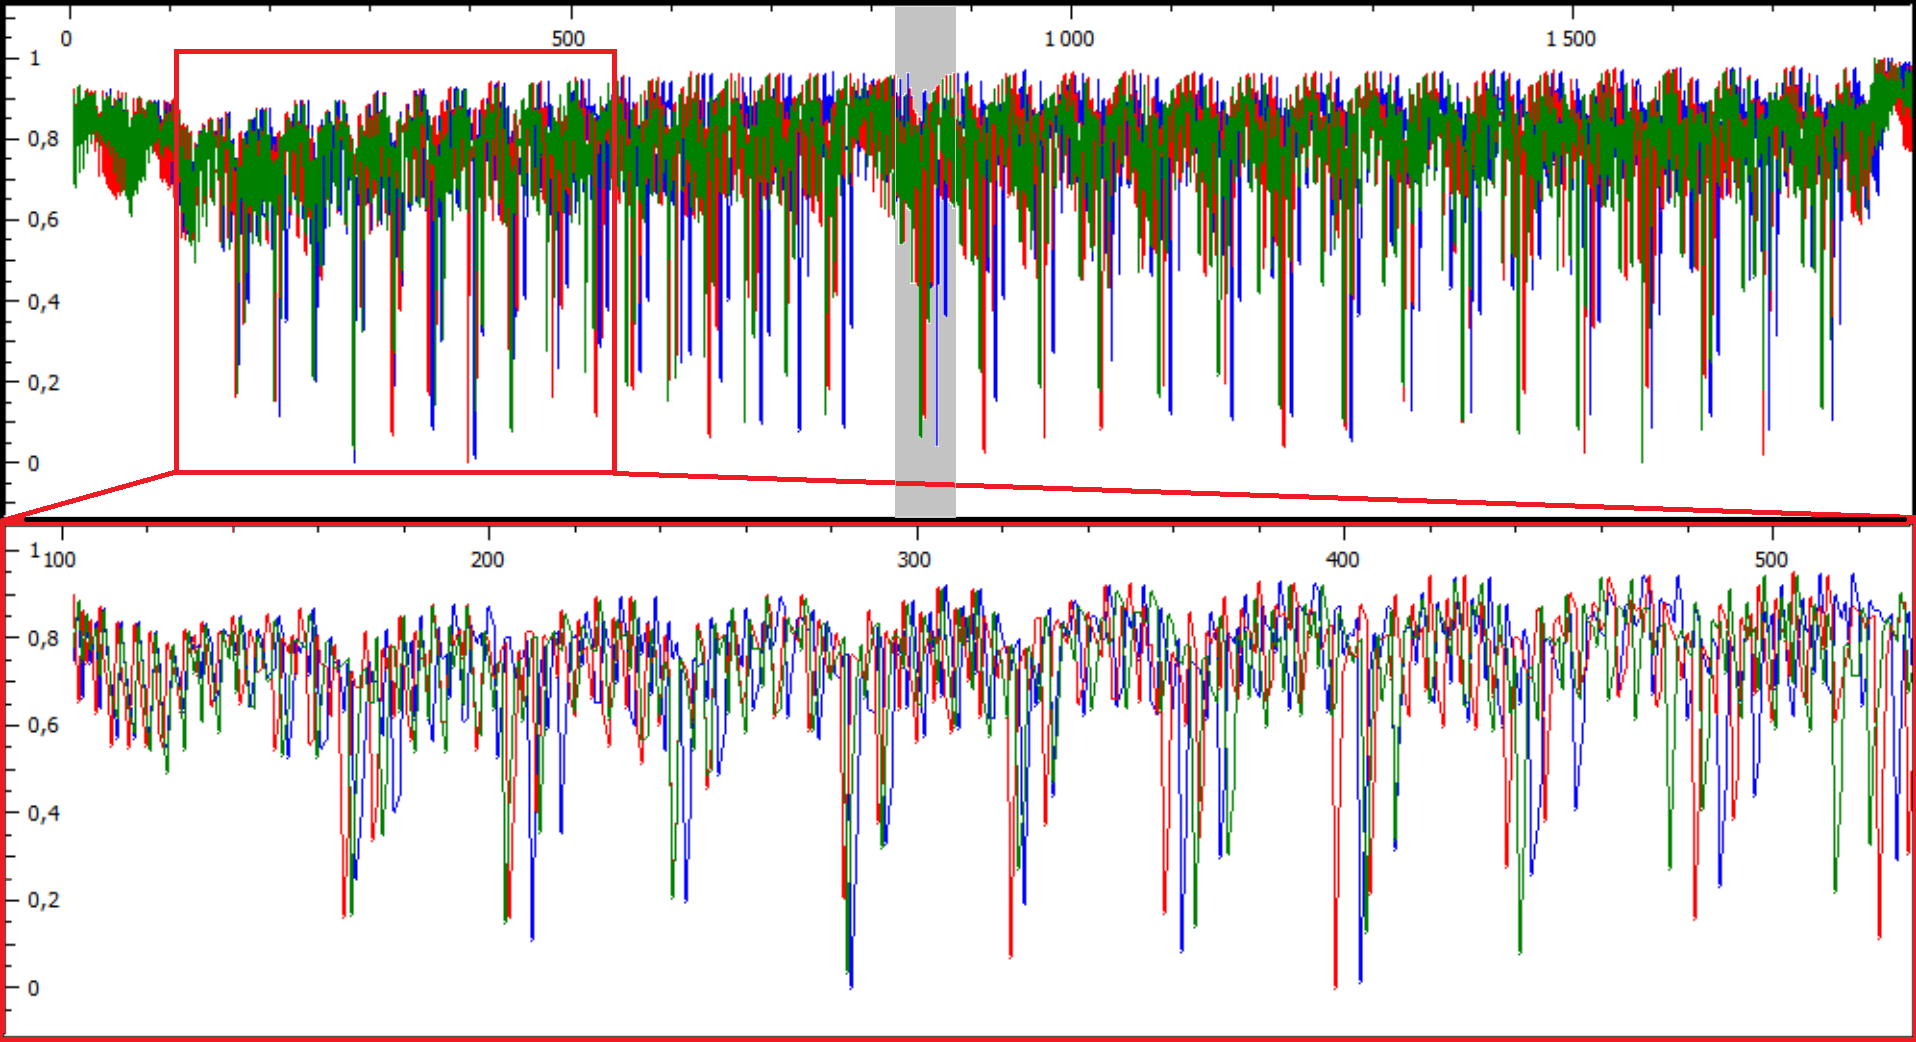
\includegraphics[width=.4\textwidth]{../Figures/CHES2017/jitter_2_2_framed.png} }
\subfloat[High artificial jitter]{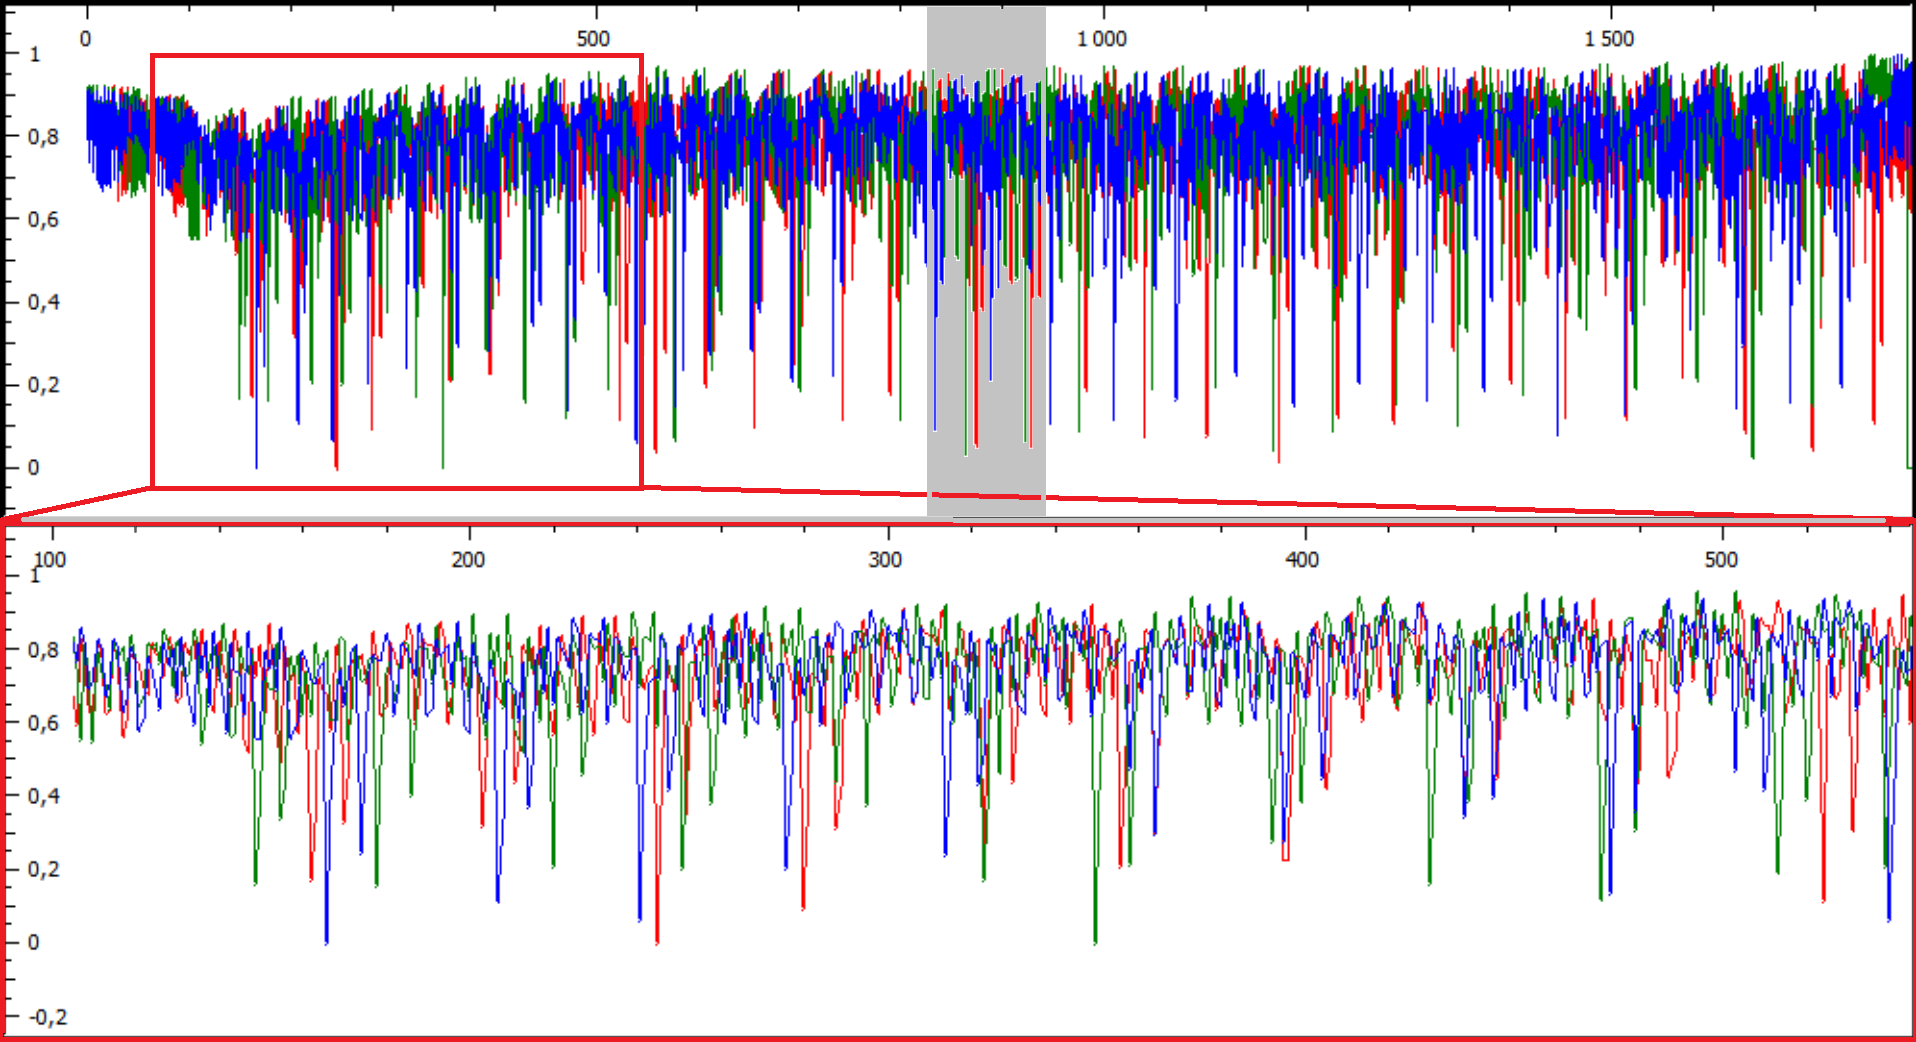
\includegraphics[width=.4\textwidth]{../Figures/CHES2017/jitter_6_6_framed.png} }
\end{figure}
\begin{block}{Target}

\begin{itemize}
\item Target Variable: $Z = \mathrm{HW}(\mathrm{Sbox}(P\oplus K))$
\item $\approx 2000$ time samples
\item Countermeasure: artificial signal treatment simulating clock jitter
\item 10000 training traces
\end{itemize}
\end{block}


\end{frame}

\begin{frame}
\frametitle{Artificial Jitter (2)}
\vspace*{-10pt}
\begin{scriptsize}
\newcolumntype{C}{>{\centering\arraybackslash}p{3em}}
\begin{table}[t]
\centering

\begin{tabular}{|C|C|CCCCCC|}
\multicolumn{8}{C}{\emph{Low\_jitter}}      \\                                            
\hline
Acc                          & $N^\star$                         & \multicolumn{2}{C|}{$\mathrm{SH}_{0}$}                                                   & \multicolumn{2}{C|}{$\mathrm{SH}_{20}$}                                                & \multicolumn{2}{C|}{$\mathrm{SH}_{40}$}                                           \\ \hline
\multicolumn{2}{|C|}{$\mathrm{AR}_{0}$}   & \multicolumn{1}{C|}{\cellcolor[HTML]{EFEFEF}57.4\%}  & \multicolumn{1}{C|}{\cellcolor[HTML]{EFEFEF}14}     & \multicolumn{1}{C|}{82.5\%}                         & \multicolumn{1}{C|}{6}                              & \multicolumn{1}{C|}{83.6\%}                                  & 6                                                            \\ \cline{1-8}
\multicolumn{2}{|C|}{$\mathrm{AR}_{100}$} & \multicolumn{1}{C|}{86.0\%}                          & \multicolumn{1}{C|}{6}                              & \multicolumn{1}{C|}{87.0\%}                         & \multicolumn{1}{C|}{5}                              & \multicolumn{1}{C|}{87.5\%}                                  & 6                                                             \\ \cline{1-8}
\multicolumn{2}{|C|}{$\mathrm{AR}_{200}$} & \multicolumn{1}{C|}{86.6\%}                          & \multicolumn{1}{C|}{6}                              & \multicolumn{1}{C|}{85.7\%} & \multicolumn{1}{C|}{6}      & \multicolumn{1}{C|}{\textbf{87.7\%}} & \textbf{5}      \\ \hline


\end{tabular}


\end{table}
\begin{table}[t]
\centering


\begin{tabular}{|C|C|CCCCCC|}
\multicolumn{8}{C}{\emph{High\_jitter}}      \\   
\hline
Acc                          & $N^\star$                         & \multicolumn{2}{C|}{$\mathrm{SH}_{0}$}                                                   & \multicolumn{2}{C|}{$\mathrm{SH}_{20}$}                                              & \multicolumn{2}{C|}{$\mathrm{SH}_{40}$}                                             \\ \hline
\multicolumn{2}{|C|}{$\mathrm{AR}_{0}$}   & \multicolumn{1}{C|}{\cellcolor[HTML]{EFEFEF}40.6\%} & \multicolumn{1}{C|}{\cellcolor[HTML]{EFEFEF}35}  & \multicolumn{1}{C|}{51.1\%} & \multicolumn{1}{C|}{9}      & \multicolumn{1}{C|}{62.4\%}           & 11                                 \\ \cline{1-8}
\multicolumn{2}{|C|}{$\mathrm{AR}_{100}$} & \multicolumn{1}{C|}{50.2\%} & \multicolumn{1}{C|}{15}     & \multicolumn{1}{C|}{72.4\%} & \multicolumn{1}{C|}{11}     & \multicolumn{1}{C|}{73.5\%}           & 9                       \\ \cline{1-8}
\multicolumn{2}{|C|}{$\mathrm{AR}_{200}$} & \multicolumn{1}{C|}{64.0\%} & \multicolumn{1}{C|}{11}     & \multicolumn{1}{C|}{\textbf{75.5\%}} & \multicolumn{1}{C|}{\textbf{8}}   & \multicolumn{1}{C|}{74.4\%}           & 8           \\ \hline


\end{tabular}


\end{table}
\end{scriptsize}


\begin{figure}
\subfloat[Low Jitter]{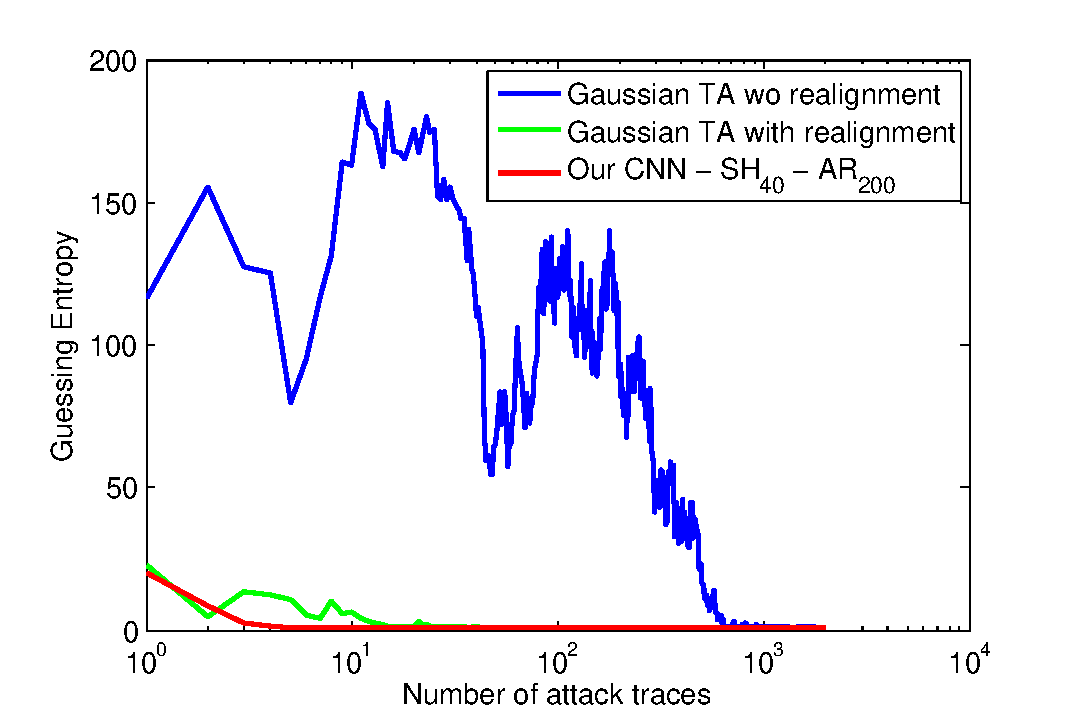
\includegraphics[width=.45\textwidth]{../Figures/CHES2017/results_low_jitter_new.pdf} }
\subfloat[High Jitter]{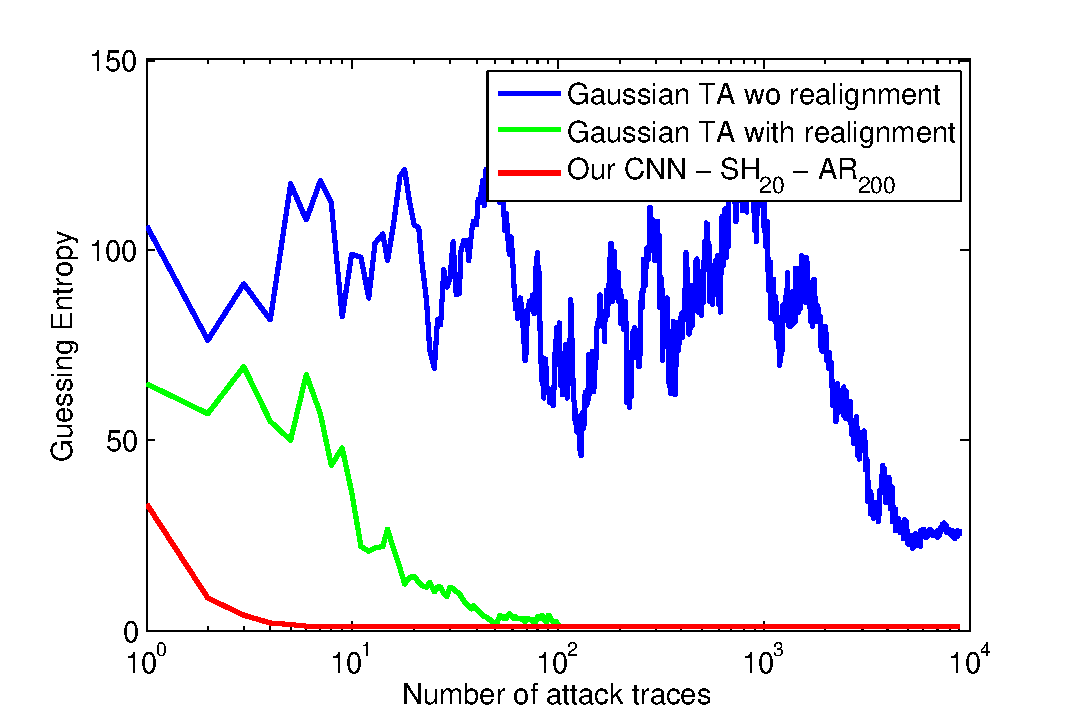
\includegraphics[width=.45\textwidth]{../Figures/CHES2017/results_high_jitter_new.pdf} }

\end{figure}
\end{frame}



\begin{frame}
\frametitle{Artificial Jitter}
\begin{tiny}

\newcolumntype{C}{>{\centering\arraybackslash}p{3em}}
\begin{table}[t]
\centering
\label{table:results_all}



\begin{tabular}{|C|C|CCCCCC|CC}
\hline
\multicolumn{10}{|C|}{\textbf{\emph{DS\_low\_jitter}}}\\
\hline
$a$                           & $b$                         & \multicolumn{2}{C|}{}                                                                                      & \multicolumn{2}{C|}{}                                                                                     & \multicolumn{2}{C|}{}                                                                                  & \multicolumn{2}{C|}{}                                      \\ \cline{1-2}
$c$                           & $d$                         & \multicolumn{2}{C|}{\multirow{-2}{*}{$\mathrm{SH}_{0}$}}                                                   & \multicolumn{2}{c|}{\multirow{-2}{*}{$\mathrm{SH}_{20}$}}                                                 & \multicolumn{2}{c|}{\multirow{-2}{*}{$\mathrm{SH}_{40}$}}                                              & \multicolumn{2}{c|}{\multirow{-2}{*}{$\mathrm{SH}_{200}$}} \\ \hline
\multicolumn{2}{|c|}{}                                      & \multicolumn{1}{c|}{\cellcolor[HTML]{EFEFEF}100.0\%} & \multicolumn{1}{c|}{\cellcolor[HTML]{EFEFEF}68.7\%} & \multicolumn{1}{c|}{99.8\%}                         & \multicolumn{1}{c|}{86.1\%}                         & \multicolumn{1}{c|}{98.9\%}                                  & 84.1\%                                  &                              &                             \\ \cline{3-8}
\multicolumn{2}{|c|}{\multirow{-2}{*}{$\mathrm{AR}_{0}$}}   & \multicolumn{1}{c|}{\cellcolor[HTML]{EFEFEF}57.4\%}  & \multicolumn{1}{c|}{\cellcolor[HTML]{EFEFEF}14}     & \multicolumn{1}{c|}{82.5\%}                         & \multicolumn{1}{c|}{6}                              & \multicolumn{1}{c|}{83.6\%}                                  & 6                                       &                              &                             \\ \cline{1-8}
\multicolumn{2}{|c|}{}                                      & \multicolumn{1}{c|}{87.7\%}                          & \multicolumn{1}{c|}{88.2\%}                         & \multicolumn{1}{c|}{82.4\%}                         & \multicolumn{1}{c|}{88.4\%}                         & \multicolumn{1}{c|}{81.9\%}                                  & 89.6\%                                  &                              &                             \\ \cline{3-8}
\multicolumn{2}{|c|}{\multirow{-2}{*}{$\mathrm{AR}_{100}$}} & \multicolumn{1}{c|}{86.0\%}                          & \multicolumn{1}{c|}{6}                              & \multicolumn{1}{c|}{87.0\%}                         & \multicolumn{1}{c|}{5}                              & \multicolumn{1}{c|}{87.5\%}                                  & 6                                       &                              &                             \\ \cline{1-8}
\multicolumn{2}{|c|}{}                                      & \multicolumn{1}{c|}{83.2\%}                          & \multicolumn{1}{c|}{88.6\%}                         & \multicolumn{1}{c|}{81.4\%} & \multicolumn{1}{c|}{86.9\%} & \multicolumn{1}{c|}{\textbf{80.6\%}} &\textbf{88.9\%} &                              &                             \\ \cline{3-8}
\multicolumn{2}{|c|}{\multirow{-2}{*}{$\mathrm{AR}_{200}$}} & \multicolumn{1}{c|}{86.6\%}                          & \multicolumn{1}{c|}{6}                              & \multicolumn{1}{c|}{85.7\%} & \multicolumn{1}{c|}{6}      & \multicolumn{1}{c|}{\textbf{87.7\%}} & \textbf{5}      &                              &                             \\ \hline
\multicolumn{2}{|c|}{}                                      &                                                      &                                                     &                                                     &                                                     &                                                              &                                         & \multicolumn{1}{c|}{85.0\%}  & \multicolumn{1}{c|}{88.6\%} \\ \cline{9-10} 
\multicolumn{2}{|c|}{\multirow{-2}{*}{$\mathrm{AR}_{500}$}} &                                                      &                                                     &                                                     &                                                     &                                                              &                                         & \multicolumn{1}{c|}{86.2\%}  & \multicolumn{1}{c|}{5}      \\ \cline{1-2} \cline{9-10}
\multicolumn{10}{|C|}{}\\
\hline
\multicolumn{10}{|C|}{\textbf{\emph{DS\_high\_jitter}}}\\
\hline
$a$                          & $b$                         & \multicolumn{2}{C|}{\multirow{2}{*}{$\mathrm{SH}_{0}$}}   & \multicolumn{2}{C|}{\multirow{2}{*}{$\mathrm{SH}_{20}$}}  & \multicolumn{2}{C|}{\multirow{2}{*}{$\mathrm{SH}_{40}$}} & \multicolumn{2}{C|}{\multirow{2}{*}{$\mathrm{SH}_{200}$}} \\ \cline{1-2}
$c$                          & $d$                         & \multicolumn{2}{C|}{}                                     & \multicolumn{2}{C|}{}                                     & \multicolumn{2}{C|}{}                                    & \multicolumn{2}{C|}{}                                     \\ \hline
\multicolumn{2}{|C|}{\multirow{2}{*}{$\mathrm{AR}_{0}$}}   & \multicolumn{1}{C|}{\cellcolor[HTML]{EFEFEF}100\%}  & \multicolumn{1}{l|}{\cellcolor[HTML]{EFEFEF}45.0\%} & \multicolumn{1}{C|}{100\%}  & \multicolumn{1}{C|}{60.0\%} & \multicolumn{1}{l|}{98.5\%}           & 67.6\%           &                             &                             \\ \cline{3-8}
\multicolumn{2}{|C|}{}                                     &  \multicolumn{1}{C|}{\cellcolor[HTML]{EFEFEF}40.6\%} & \multicolumn{1}{C|}{\cellcolor[HTML]{EFEFEF}35}  & \multicolumn{1}{C|}{51.1\%} & \multicolumn{1}{C|}{9}      & \multicolumn{1}{C|}{62.4\%}           & 11               &                             &                             \\ \cline{1-8}
\multicolumn{2}{|C|}{\multirow{2}{*}{$\mathrm{AR}_{100}$}} & \multicolumn{1}{C|}{90.4\%} & \multicolumn{1}{l|}{57.3\%} & \multicolumn{1}{C|}{76.6\%} & \multicolumn{1}{C|}{73.6\%} & \multicolumn{1}{C|}{78.5\%}           & 76.4\%           &                             &                             \\ \cline{3-8}
\multicolumn{2}{|C|}{}                                     & \multicolumn{1}{C|}{50.2\%} & \multicolumn{1}{C|}{15}     & \multicolumn{1}{C|}{72.4\%} & \multicolumn{1}{C|}{11}     & \multicolumn{1}{C|}{73.5\%}           & 9                &                             &                             \\ \cline{1-8}
\multicolumn{2}{|C|}{\multirow{2}{*}{$\mathrm{AR}_{200}$}} & \multicolumn{1}{C|}{83.1\%} & \multicolumn{1}{C|}{67.7\%} &\multicolumn{1}{C|}{\textbf{82.0\%}} & \multicolumn{1}{C|}{\textbf{77.1\%}} & \multicolumn{1}{l|}{82.6\%}           & 77.0\%           &                             &                             \\ \cline{3-8}
\multicolumn{2}{|C|}{}                                     & \multicolumn{1}{C|}{64.0\%} & \multicolumn{1}{C|}{11}     & \multicolumn{1}{C|}{\textbf{75.5\%}} & \multicolumn{1}{C|}{\textbf{8}}   & \multicolumn{1}{C|}{74.4\%}           & 8                &                             &                             \\ \hline
\multicolumn{2}{|C|}{\multirow{2}{*}{$\mathrm{AR}_{500}$}} &                             &                             &                             &                             &                                       &                  & \multicolumn{1}{C|}{83.6\%} & \multicolumn{1}{C|}{73.4\%} \\ \cline{9-10} 
\multicolumn{2}{|C|}{}                                     &                             &                             &                             &                             &                                       &                  & \multicolumn{1}{C|}{68.2\%} & \multicolumn{1}{C|}{11}     \\ \cline{1-2} \cline{9-10}  
\end{tabular}


\end{table}

\end{tiny}
\end{frame}

\begin{frame}
\frametitle{Real Jitter (1)}
\vspace{-10pt}
\begin{block}{Target}
\begin{itemize}
\item AES hardware implementation
\item strong jitter effect
\item Target Variable: $Z = \mathrm{Sbox}(P\oplus K)$
\item $2,500$ selected time samples
\item $99,000$ training traces
\end{itemize}
\end{block}

\only<1>{
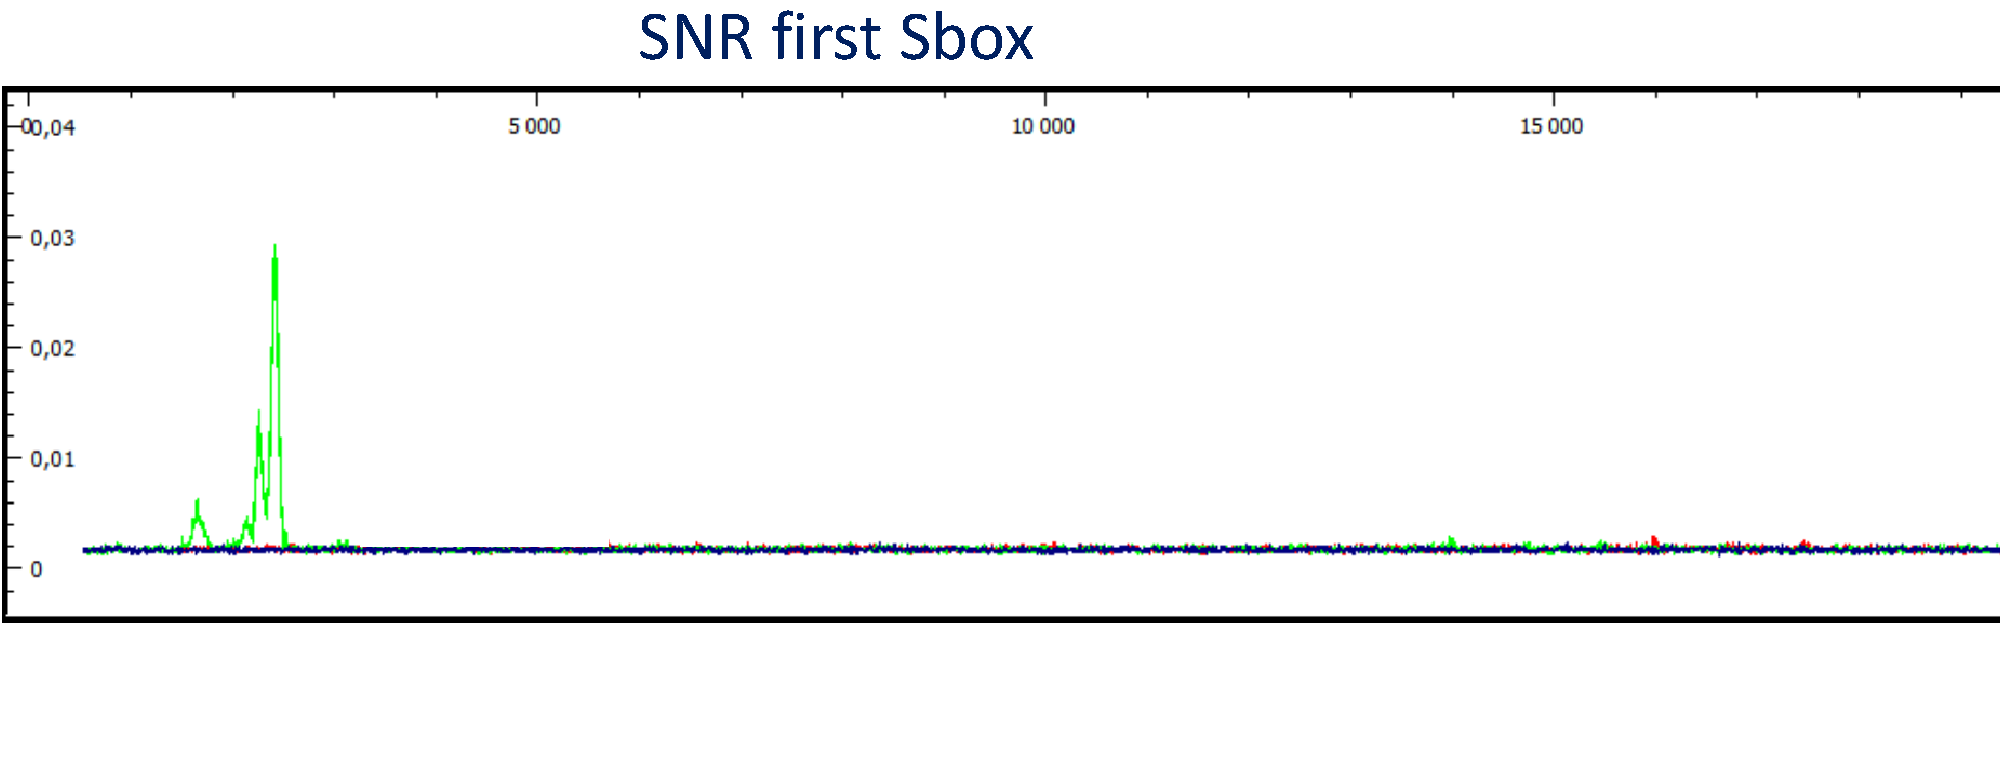
\includegraphics[width=\textwidth]{../Figures/CHES2017/SNR_firstSbox.pdf}
}
\only<2>{
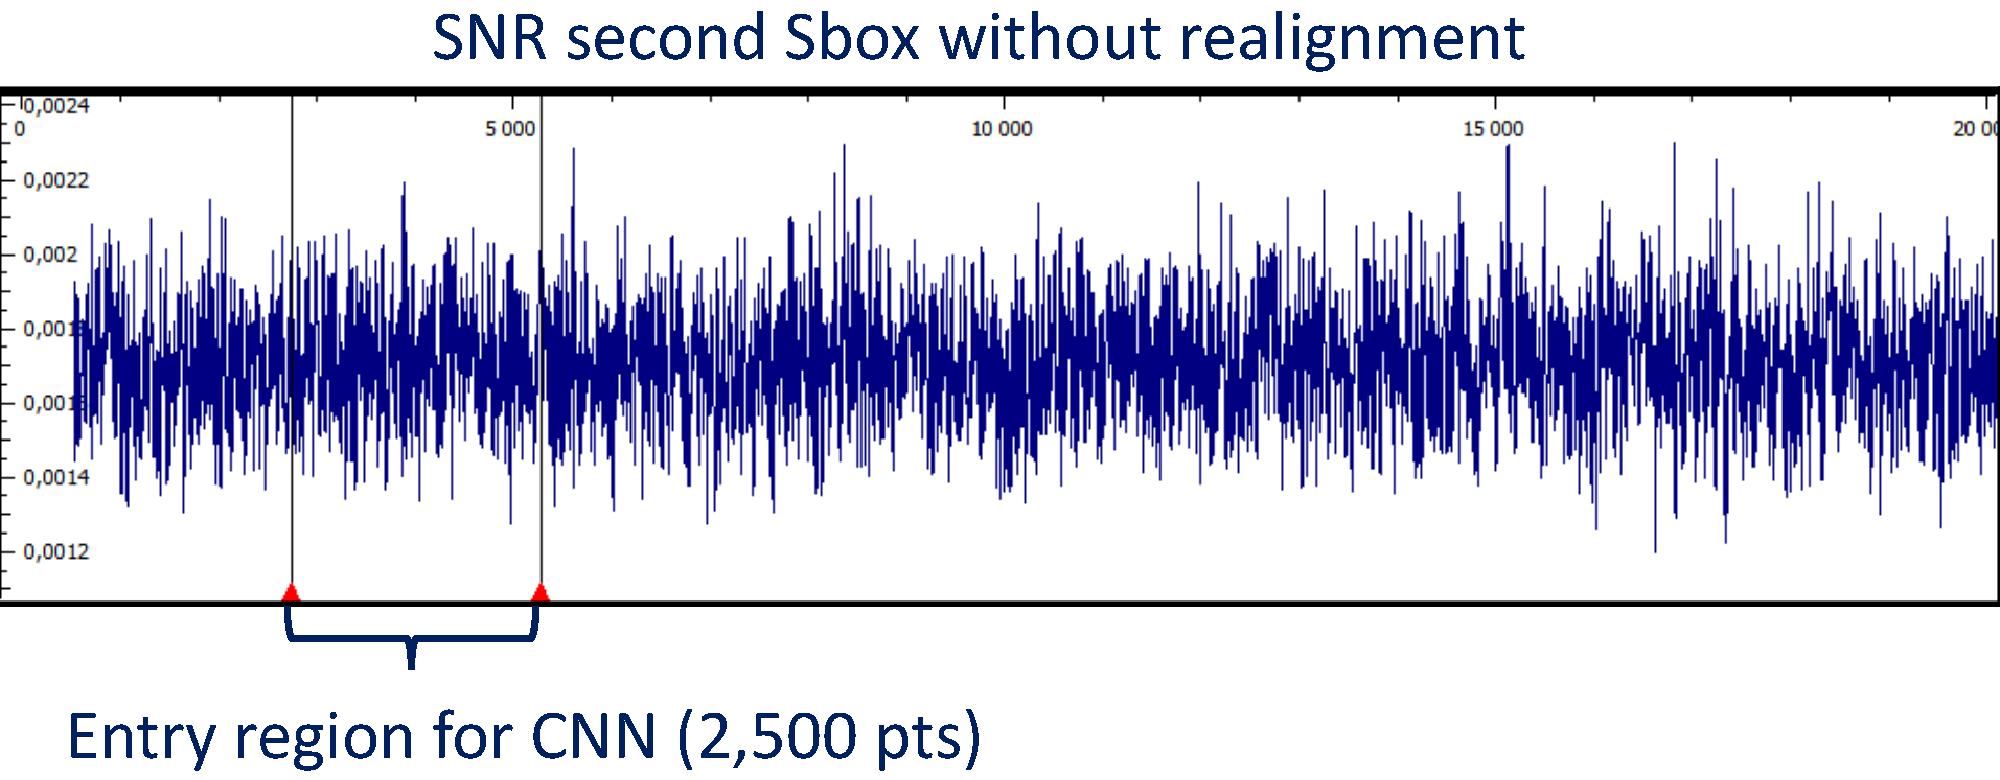
\includegraphics[width=\textwidth]{../Figures/CHES2017/SNR_desynchro.pdf}
}



\end{frame}

\begin{frame}
\frametitle{Real Jitter (2)}
\centering
\begin{scriptsize}
\begin{table}
\begin{tabular}{|c|c|c|c|c|c|c|c|}
\multicolumn{8}{c}{}\\
\hline
\multicolumn{2}{|c|}{} & \multicolumn{2}{c|}{\textcolor{green}{$\mathrm{SH}_{0}$}\textcolor{blue}{$\mathrm{AR}_{0}$}} & \multicolumn{2}{c|}{\textcolor{green}{$\mathrm{SH}_{10}$}\textcolor{blue}{$\mathrm{AR}_{100}$}} & \multicolumn{2}{c|}{\textcolor{green}{$\mathrm{SH}_{20}$}\textcolor{blue}{$\mathrm{AR}_{200}$}} \\ \hline
Acc        & $N^\star$       & 1.2\%                      & 137                      & 1.3\%                       & 89                         & \textbf{1.8\%}              & \textbf{54}                \\ \hline
\end{tabular}
\end{table}
\end{scriptsize}
\uncover<2>{
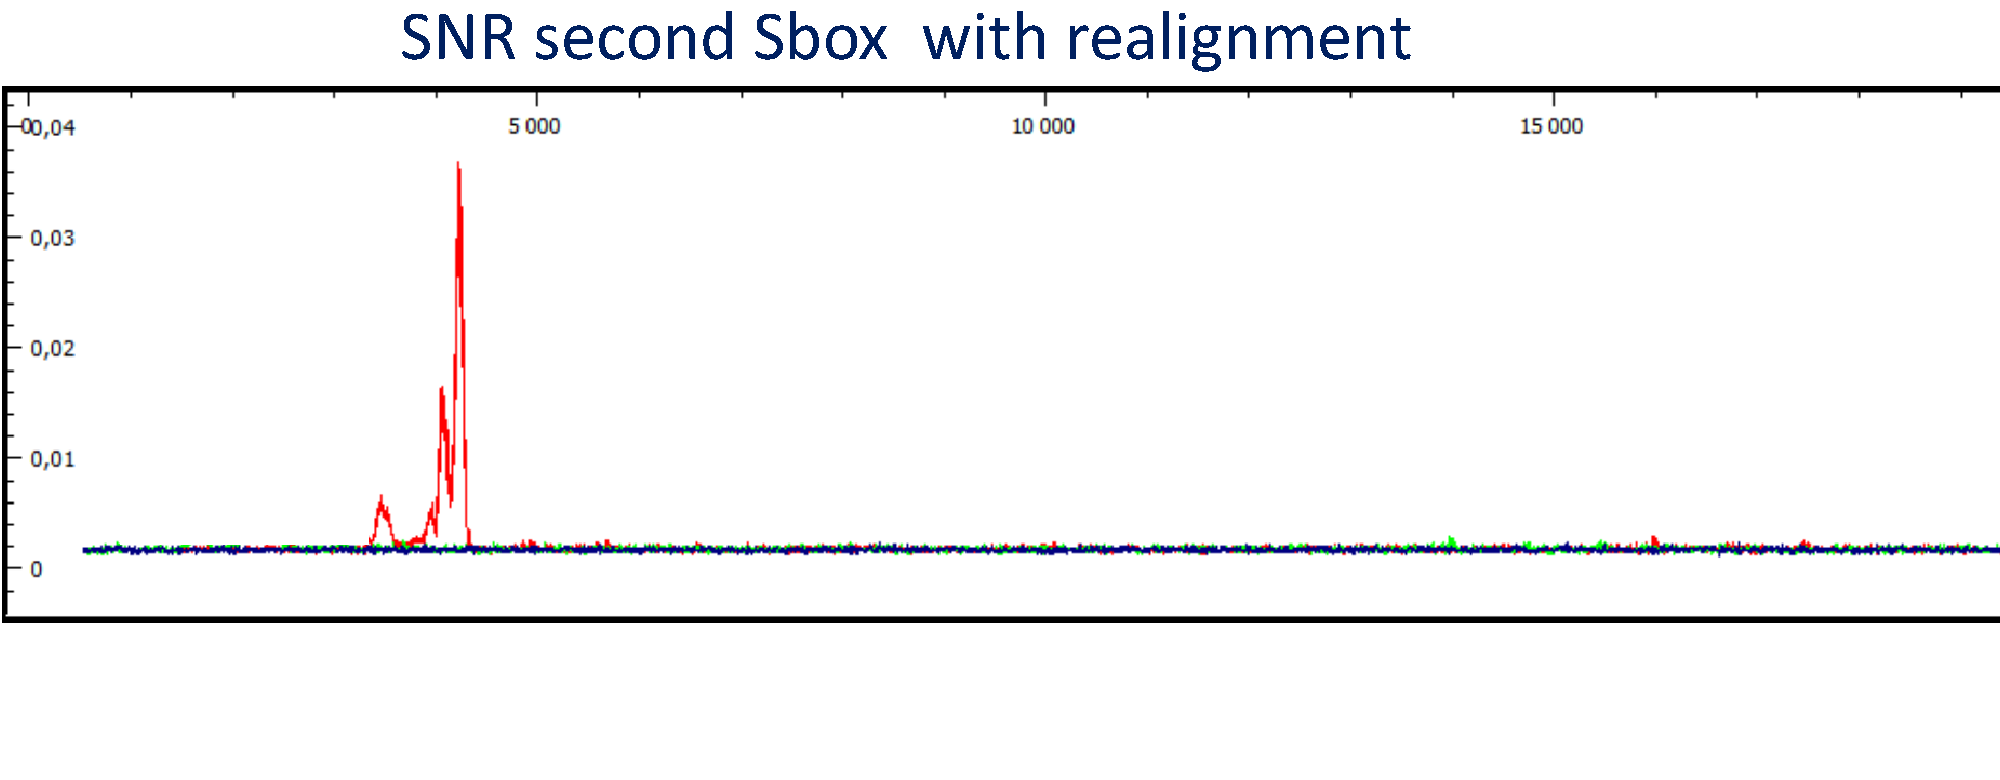
\includegraphics[width=0.75\textwidth]{../Figures/CHES2017/SNR_resynchro.pdf} 
}
\vspace*{-18pt}

\centering
\uncover<2>{
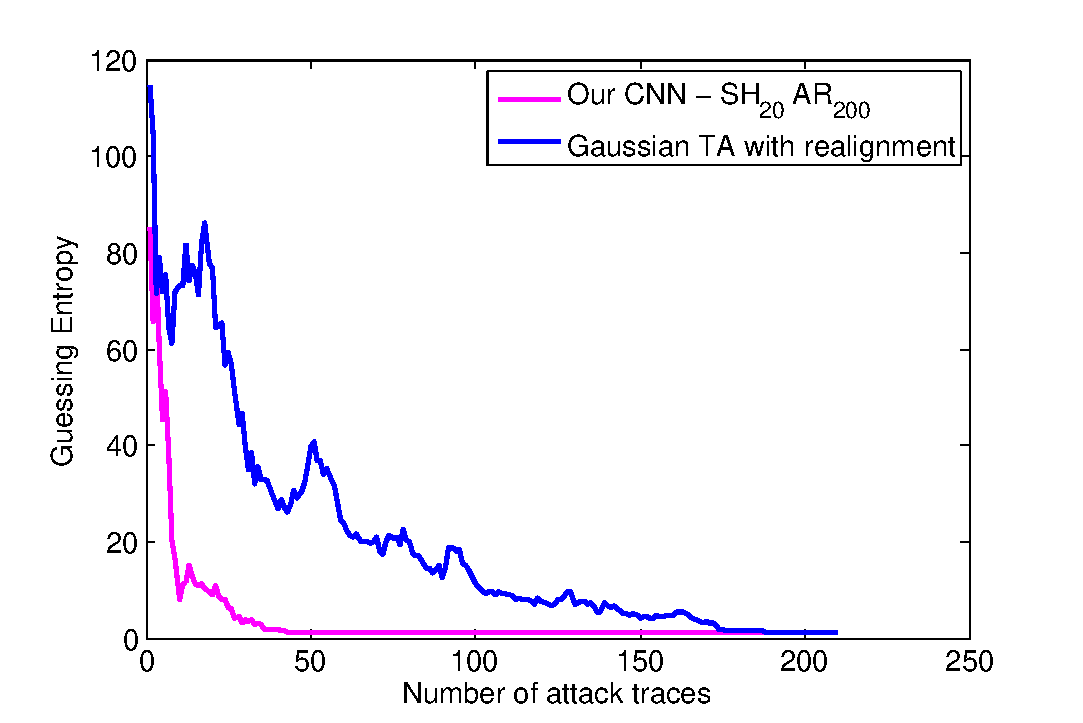
\includegraphics[width=0.5\textwidth]{../Figures/CHES2017/TA_CNN_smartcard.pdf} 
}


\end{frame}

\begin{frame}
\frametitle{Conclusions about CNN}

\begin{block}{}
\begin{itemize}
\item State-of-the-Art Template Attack routine separates resynchronization/dimensionality reduction from characterization \pause
\item CNNs provide an integrated approach to directly construct a discriminative model from rough data \pause
\item CNN models may have high capacity and require plenty of data to be trained \pause 
\item Data Augmentation provides an answer to the lack of data \pause
\item we proposed two Side-Channel-adapted Data Augmentation techniques (inspired by trace misalignment)\pause
\item we verified the effectiveness/efficiency of the CNN+Data Augmentation approach over different sets of misaligned data
\end{itemize}
\end{block}

\end{frame}
